% !TEX program = xelatex
% Dòng trên báo cho VS Code (LaTeX Workshop) biên dịch bằng XeLaTeX thay vì pdfLaTeX; gói fontspec (font tiếng Việt)
% chỉ chạy với XeLaTeX hoặc LuaLaTeX. latexmk đọc cấu hình trong latexmkrc cùng thư mục.
% Báo cáo đồ án FPClose theo mẫu IEEE conference (IEEEtran). Biên dịch tay (tiếng Việt):
%   cd docs/IEEE-conference-template-062824
%   xelatex report.tex && xelatex report.tex
% Hình lấy từ results/figures/ (sinh bởi scripts/make_figures.jl), bảng từ tables/ (cùng script).
% Ba chương nằm trong chuong1.tex, chuong2.tex, chuong3.tex; Chương 1 và 3 hiện là khung (\todo màu đỏ).
\documentclass[conference]{IEEEtran}
\IEEEoverridecommandlockouts

% Toàn bộ báo cáo dùng Times New Roman: chữ thường, chữ không chân và chữ đơn cách (đường dẫn file, tên hàm) đều là
% Times New Roman; công thức toán dùng Times của gói mathptmx. Máy không có Times New Roman thì dùng TeX Gyre Termes
% (bản Times mã nguồn mở đi kèm MiKTeX/TeX Live). Chữ trong hình cũng là Times New Roman (scripts/make_figures.jl).
\usepackage{amsmath,amssymb,amsfonts}
\usepackage{mathptmx}
\usepackage[no-math]{fontspec}   % no-math: giữ font toán Times của mathptmx cho số và dấu = + ( )
\IfFontExistsTF{Times New Roman}{\newcommand{\reportfont}{Times New Roman}}{\newcommand{\reportfont}{TeX Gyre Termes}}
\setmainfont{\reportfont}
\setsansfont{\reportfont}
\setmonofont{\reportfont}
% Dấu đầu dòng lấy từ font chữ (Times New Roman) thay cho ký hiệu toán \bullet của IEEEtran
\renewcommand{\labelitemi}{\textbullet}
\usepackage{graphicx}
\usepackage{adjustbox}
\usepackage{array}       % cột p{} căn trái trong bảng độ phức tạp (Mục 2.8)
\usepackage{etoolbox}    % \patchcmd: sửa kiểu chú thích bảng bên dưới
\usepackage{float}       % [H]: bảng, hình của Phụ lục A đứng đúng chỗ, không trôi sang Phụ lục B, C
\usepackage{url}
\usepackage{xcolor}
% Liên kết bấm được trong PDF: \cite{...} nhảy tới Tài liệu tham khảo, \ref{...} tới hình, bảng, mục; \url{...} trỏ đúng
% địa chỉ đầy đủ kể cả khi bị ngắt dòng. Link tô màu xanh đậm để dễ thấy chỗ bấm được; muốn chữ đen hoàn toàn (kiểu IEEE
% thuần) thì thay \hypersetup bên dưới bằng \hypersetup{hidelinks}. Bookmark (mục lục bên trái trình đọc PDF) hiện
% "Chương 1: ...", "Chương 2: ...", "Chương 3: ...". hyperref phải nạp sau cùng.
\usepackage{hyperref}
\definecolor{linkblue}{RGB}{0,51,153}
\hypersetup{colorlinks=true, linkcolor=linkblue, citecolor=linkblue, urlcolor=linkblue,
            bookmarksopen=true, bookmarksopenlevel=1,
            pdftitle={Cài đặt và đánh giá thuật toán FPClose khai thác tập phổ biến đóng}}

\graphicspath{{../../results/figures/}}
% Đường dẫn file viết bằng \path{...} (gói url): cho ngắt dòng sau / _ . - để không làm giãn chữ cả dòng
\renewcommand{\UrlBreaks}{\do\/\do\_\do\.\do\-}
\renewcommand{\UrlFont}{\ttfamily\small}
\renewcommand{\figurename}{Hình}
\renewcommand{\tablename}{Bảng}
\renewcommand{\refname}{Tài liệu tham khảo}
\renewcommand{\abstractname}{Tóm tắt}

\renewcommand{\IEEEkeywordsname}{Từ khóa}
\renewcommand{\appendixname}{Phụ lục}

% Báo cáo gồm 3 chương theo đề (mỗi chương là một \section). Đánh số theo kiểu bài báo gốc (Grahne & Zhu, TKDE 2005):
% chương "Chương 2.", mục "2.3", mục con "2.3.1"; tham chiếu \ref tới mục hiện đúng số đó.
% \todo{...}: chỗ còn phải viết, in chữ đỏ để dễ thấy; xóa hết trước khi nộp
\newcommand{\todo}[1]{{\color{red}\itshape [Cần viết: #1]}}

% Tiêu đề chương: IEEEtran dùng chữ hoa nhỏ (\scshape), Times New Roman không có kiểu này nên chữ to nhỏ lẫn lộn;
% đổi thành chữ đậm, cùng một cỡ (giữ nguyên khoảng cách của IEEEtran)
\makeatletter
% Chú thích bảng: IEEEtran in chữ hoa nhỏ (\scshape), làm ký hiệu toán và tiếng Việt bị đổi dạng (R_tree thành R_TREE);
% bỏ \scshape để chú thích bảng dùng chữ thường như chú thích hình
\patchcmd{\@makecaption}{\normalfont\footnotesize\scshape #2}{\normalfont\footnotesize #2}{}{\PackageWarning{report}{Không sửa được chú thích bảng}}
\def\section{\@startsection{section}{1}{\z@}{1.5ex plus 1.5ex minus 0.5ex}%
{0.7ex plus 1ex minus 0ex}{\normalfont\normalsize\centering\bfseries}}
% Tiêu đề chương in hoa toàn bộ; bookmark PDF vẫn giữ chữ thường
\let\IEEEsection\section
\renewcommand{\section}{\@ifstar{\upsecstar}{\upsec}}
\newcommand{\upsecstar}[1]{\IEEEsection*{\MakeUppercase{#1}}}
\newcommand{\upsec}[1]{\IEEEsection[#1]{\MakeUppercase{#1}}}
\makeatother

\renewcommand{\thesection}{\arabic{section}}
\renewcommand{\thesectiondis}{CHƯƠNG~\thesection.}
\renewcommand{\thesubsection}{\thesection.\arabic{subsection}}
\renewcommand{\thesubsectiondis}{\thesubsection}
\renewcommand{\thesubsubsection}{\thesubsection.\arabic{subsubsection}}
\renewcommand{\thesubsubsectiondis}{\thesubsubsection}

% \colfig{file}{chú thích}{nhãn}: một biểu đồ vừa một cột, như các hình của bài báo gốc (mỗi hình một CSDL)
\newcommand{\colfig}[3]{\begin{figure}[!t]\centering\includegraphics[width=\columnwidth]{#1}\caption{#2}\label{#3}%
\end{figure}}
% Cho phép nhiều hình nhỏ trên một trang, để hình đứng gần đoạn văn nhắc tới chúng
\setcounter{topnumber}{3}
\setcounter{bottomnumber}{2}
\setcounter{totalnumber}{5}
\renewcommand{\topfraction}{0.9}
\renewcommand{\bottomfraction}{0.6}
\renewcommand{\textfraction}{0.1}
\renewcommand{\floatpagefraction}{0.8}
\renewcommand{\dbltopfraction}{0.9}
\renewcommand{\dblfloatpagefraction}{0.8}

% \fittable{độ rộng tối đa}{tên bảng trong tables/}: chỉ thu nhỏ khi bảng rộng hơn khổ, không phóng to
% (chữ cỡ footnotesize, khoảng cách cột hẹp để bảng ít bị thu nhỏ)
\newcommand{\fittable}[2]{\begin{adjustbox}{max width=#1}\footnotesize\setlength{\tabcolsep}{3.5pt}%
\input{tables/#2}\end{adjustbox}}

\begin{document}

\title{Cài đặt và đánh giá thuật toán FPClose khai thác tập phổ biến đóng}

\author{\IEEEauthorblockN{Nhóm FPClose}
\IEEEauthorblockA{Khoa Công nghệ Thông tin, Trường Đại học Khoa học Tự nhiên, ĐHQG-HCM}}

\maketitle

\begin{abstract}
Báo cáo trình bày việc cài đặt lại từ đầu bằng Julia thuật toán FPClose của Grahne và Zhu 
để khai thác tập phổ biến đóng, kèm bước khôi phục mọi tập phổ biến và sinh luật kết hợp. Tính đúng
đắn được kiểm chứng bằng bộ kiểm thử tự động, gồm cả đối chiếu với đáp án vét cạn, và bằng phép so từng itemset với
SPMF: kết quả khớp hoàn toàn trên 56/56 cấu hình minsup của chín CSDL benchmark.
Về thời gian, trên cùng một máy và với thời gian gồm đọc dữ liệu, khai thác, ghi kết quả nhưng không gồm khởi động JVM
hay Julia, cài đặt của nhóm nhanh hơn SPMF ở 44/56 cấu hình (tỉ số thời gian nhóm/SPMF dưới 0,90), rõ nhất trên dữ liệu
dày. Phía nhóm được warm-up trước khi đo còn SPMF chạy trên JVM mới, nên lợi thế ở các cấu hình chạy rất nhanh có thể
bị phóng đại. Thực nghiệm còn
đánh giá bộ nhớ, đóng góp của từng tối ưu, khả năng mở rộng và ảnh hưởng của độ dài giao dịch. Chương 3 áp dụng cài đặt vào hai bài toán: phân tích giỏ hàng trên UCI Online Retail, nơi các luật nổi bật cho thấy khách hàng thường mua nhiều biến thể của cùng một bộ sưu tập; và khai thác mẫu visual word trên ảnh Caltech-101, nơi các tập đóng hỗ trợ phân tích mẫu đặc trưng của từng lớp nhưng chưa cải thiện rõ độ chính xác phân loại.
\end{abstract}

\begin{IEEEkeywords}
Khai thác dữ liệu, tập phổ biến đóng, FPClose, FP-tree, luật kết hợp, Julia.
\end{IEEEkeywords}

\section{\texorpdfstring{Cài đặt}{CHƯƠNG 1: CÀI ĐẶT}}
\label{sec:implementation}

Khai thác tập phổ biến là bước nền của khai thác luật kết hợp, nhưng số tập phổ biến tăng bùng nổ khi minsup giảm: trên
mushrooms ở minsup 20\% đã có 53\,583 tập phổ biến, trong khi chỉ có 1\,197 tập phổ biến đóng. Có hai cách biểu diễn nén
thường dùng là tập phổ biến tối đại (\textit{maximal itemset}: tập phổ biến không có tập cha nào phổ biến) và tập phổ
biến đóng, với quan hệ tập tối đại $\subseteq$ tập đóng $\subseteq$ tập phổ biến. Tập tối đại gọn hơn nhưng làm mất
thông tin: từ chúng chỉ biết được những tập nào phổ biến, không biết support của các tập đó, nên không tính được confidence của luật kết hợp. Ngược lại, tập đóng là biểu diễn nén \emph{không mất thông tin}: từ các tập
đóng cùng support của chúng có thể suy ra mọi tập phổ biến và support tương ứng. Vì vậy, tập đóng phù hợp với các bài toán cần support chính xác của mọi tập phổ biến, tiêu biểu là sinh luật kết hợp. Trong các thuật toán khai thác tập đóng,
nhóm chọn FPClose~\cite{grahne2005} vì thuật toán khai thác trực tiếp trên FP-tree mà không sinh ứng viên, kiểm tra tính
đóng bằng một cấu trúc cây cục bộ thay vì so với toàn bộ các tập đã tìm, và có kỹ thuật FP-array giúp giảm số lần duyệt
cây trên dữ liệu thưa. Thuật toán được cài đặt lại từ đầu bằng Julia 1.13.4; ngôn ngữ này biên dịch JIT theo kiểu cụ
thể (\textit{concrete type}) nên cho hiệu năng gần ngôn ngữ biên dịch tĩnh, trong khi mã nguồn vẫn ngắn gọn và gần với
mã giả. Mục~\ref{sec:algorithm} tóm tắt thuật toán theo bài báo gốc, các mục tiếp theo lần lượt trình bày cài đặt cơ
bản, kiểm thử, tối ưu, giao diện dòng lệnh và những điểm khác với bài báo.

\textit{Support} của một itemset $X$, ký hiệu $\sigma(X)$, là số giao dịch chứa $X$. Itemset $X$ là tập phổ biến
(\textit{frequent itemset}) nếu $\sigma(X)$ không nhỏ hơn ngưỡng minsup, và là tập phổ biến đóng (\textit{closed
itemset}) nếu không có tập cha thực sự nào có cùng support~\cite{pasquier1999}. FPClose chỉ xuất các tập đóng; support
của mọi tập phổ biến $Y$ được suy ra bằng
\begin{equation}
  \sigma(Y) = \max\{\sigma(C) : C \text{ đóng},\ Y \subseteq C\}.
  \label{eq:recovery}
\end{equation}

\subsection{Thuật toán FPClose}
\label{sec:algorithm}

\textbf{FP-tree và cây điều kiện.} FPClose~\cite{grahne2005} dựng FP-tree~\cite{han2000} (\textit{frequent-pattern
tree}: cây tiền tố gộp các giao dịch có chung phần đầu, mỗi nút lưu một item và số giao dịch đi qua) bằng hai lần quét
CSDL: lần thứ nhất đếm support của từng item, lần thứ hai chèn mỗi giao dịch, sau khi bỏ item không phổ biến và sắp xếp
theo support giảm dần, vào cây. Bảng header của cây lưu các item theo cùng thứ tự, kèm danh sách liên kết
(\textit{node-link}) nối mọi nút của cùng một item. Với một cây $T_X$ của itemset cơ sở $X$ và một item $i$ trong
header, các đường đi từ những nút của $i$ lên gốc tạo thành \textit{pattern base} của $X \cup \{i\}$; cây dựng từ
pattern base này là cây điều kiện (\textit{conditional FP-tree}) $T_{X \cup \{i\}}$, và thuật toán đệ quy trên cây đó.

\textbf{CFI-tree và kiểm tra tính đóng.} Vì FPClose duyệt theo chiều sâu và xử lý các item trong header theo thứ tự
support \emph{tăng dần}, một tập phổ biến mới tìm được chỉ có thể là tập con của một tập đóng đã tìm trước đó. Các tập
đóng đã tìm được lưu trong CFI-tree (\textit{closed frequent itemset tree}), một biến thể của FP-tree. Mỗi CFI-tree
$C_X$ gắn với một cây $T_X$, dùng cùng thứ tự item với header của $T_X$ và chỉ chứa các tập đóng đã tìm có chứa $X$.
Mỗi nút có bốn trường: item, count, node-link và level (độ sâu của nút). Khi chèn một tập đóng, count của nút không được
cộng dồn như FP-tree mà được thay bằng giá trị lớn nhất. Hàm \texttt{closed\_checking}$(Y, C)$ với
$Y = \{i_1, \ldots, i_k\}$ có support $c$ đi theo node-link của $i_k$; với mỗi nút có count $\geq c$, hàm kiểm tra $Y$
có là tập con của các tổ tiên của nút đó không, và dùng level để dừng sớm khi số tổ tiên còn lại ít hơn số item cần
khớp. $Y$ không đóng khi tồn tại một tập đóng $Z \supset Y$ trong $C$ có cùng support.

\textbf{Thuật toán.} Hình~\ref{fig:fpclose} là mã giả FPClose theo cài đặt
của nhóm, dựa trên Fig.~8 của bài báo gốc. Nếu cây chỉ có một nhánh, các
tập đóng ứng viên được đọc trực tiếp từ nhánh: tại mỗi vị trí support giảm,
phần đầu nhánh ghép với $X$ tạo thành một ứng viên (dòng 1--3). Ngược lại,
thuật toán xét lần lượt từng item $i$ trong header, từ item ít phổ biến nhất.
Nhánh của $i$ chỉ sinh các tập dạng $Y \cup W$, với $Y = X \cup \{i\}$ và $W$ gồm các item xếp trước $i$ trong header.
Giả sử đã có tập đóng $Z \supsetneq Y$ cùng support với $Y$. Khi đó mọi giao dịch chứa $Y$ đều chứa $Z$, nên
$Y \cup W$ và $Y \cup W \cup Z$ có cùng support. Vì $Z$ được tìm trước, nó chứa ít nhất một item đã được xử lý ở bước
trước và không thể thuộc $W$; do đó mọi $Y \cup W$ đều không đóng, và nhánh được cắt mà không mất kết quả (dòng 7).
Lập luận này dựa vào thứ tự duyệt: nói chung, tập cha của một tập không đóng vẫn có thể đóng. Nếu không bị cắt, thuật
toán dựng cây điều kiện $T_Y$ và CFI-tree $C_Y$ rồi đệ quy (dòng 8--9). Cuối
mỗi lời gọi, $X$ được ghi nhận nếu chưa bị bao trùm (dòng 10). Mỗi tập đóng
mới được thêm ngay vào các CFI-tree đang dùng (thủ tục Record), để các nhánh
xét sau kiểm tra được.

% Mã giả viết bằng tabular (template không nạp gói algorithm). \ii{n}: thụt n em, dòng bị ngắt cũng thụt theo.
\begin{figure}[t]
\centering
\footnotesize
\newcommand{\ii}[1]{\hangindent=\dimexpr#1em+1.5em\relax\hangafter=1\hspace*{#1em}}
\begin{tabular}{@{}r@{\;\;}>{\raggedright\arraybackslash}p{\dimexpr\columnwidth-2.2em\relax}@{}}
\multicolumn{2}{@{}>{\raggedright\arraybackslash}p{\columnwidth}@{}}{\textbf{Thủ tục} FPClose$(T, C)$ \quad
$X$: tập cơ sở (tiền tố) gắn với $T$, $X = \varnothing$ ở lời gọi đầu; \ $T$: FP-tree có điều kiện của $X$; \
$C$: CFI-tree của $X$}\\[2pt]
1 & \ii{0}\textbf{if} $T$ chỉ có một nhánh \textbf{then}\\
2 & \ii{1}\textbf{for} mỗi đoạn đầu nhánh $Z$ có support khác item kế tiếp \textbf{do}\\
3 & \ii{2}\textbf{if} $X \cup Z$ chưa bị bao bởi tập đóng nào đã tìm thấy \textbf{then} Record$(X \cup Z)$\\
4 & \ii{0}\textbf{else}\\
5 & \ii{1}\textbf{for} mỗi item $i$ trong header của $T$, từ ít phổ biến nhất \textbf{do}\\
6 & \ii{2}$Y \gets X \cup \{i\}$\\
7 & \ii{2}\textbf{if} $Y$ đã bị bao bởi tập đóng cùng support \mbox{\textbf{then continue}}%
\nobreak\hspace{0pt plus 1filll}\penalty50\hspace*{1em}\hbox{}\nobreak\hspace{0pt plus 1filll}%
\mbox{$\triangleright$ cắt nhánh}\\
8 & \ii{2}dựng $T_Y$ từ pattern base của $i$; \ $C_Y \gets$ các tập đóng trong $C$ chứa $i$\\
9 & \ii{2}FPClose$(T_Y, C_Y)$\\
10 & \ii{0}\textbf{if} $X$ chưa bị bao bởi tập đóng cùng support \textbf{then} Record$(X)$\\[3pt]
\multicolumn{2}{@{}>{\raggedright\arraybackslash}p{\columnwidth}@{}}{\textbf{Thủ tục} Record$(Z)$: thêm $Z$ vào kết
quả và vào các CFI-tree đang dùng (count các nút lấy max).}\\
\end{tabular}
\caption{Mã giả FPClose theo cài đặt của nhóm, dựa trên Fig.~8 của~\cite{grahne2005}. ``Bị bao'' nghĩa là CFI-tree đã
chứa một tập đóng bao $Z$ với cùng support. Các tối ưu tùy chọn và điểm khác bài báo xem
Mục~\ref{sec:optimizations} và~\ref{sec:deviations}.}
\label{fig:fpclose}
\end{figure}

\textbf{Ví dụ.} Xét CSDL gồm năm giao dịch $\{a,b,c,e\}$, $\{a,d,e\}$, $\{a,d\}$, $\{a,c,d\}$, $\{b,c,e\}$ với minsup
bằng 2 giao dịch. CSDL có 12 tập phổ biến nhưng chỉ 7 tập đóng: $a{:}4$, $c{:}3$, $e{:}3$, $ac{:}2$, $ad{:}3$, $ae{:}2$
và $bce{:}2$, trong đó 4 tập là tối đại ($ac$, $ad$, $ae$, $bce$). Chẳng hạn $d$ không đóng vì mọi giao dịch chứa $d$ đều chứa $a$ ($\sigma(ad) = \sigma(d) = 3$), và theo
\eqref{eq:recovery}, $\sigma(d) = \sigma(ad) = 3$. Với thứ tự header $a, c, d, e, b$, item $b$ được xử lý đầu tiên và
cho tập đóng $bce{:}2$. Cây điều kiện của $e$ có hai nhánh, với header $a, c$; khi xét $c$ trước, tập $Y = ce$ có support
2, \texttt{closed\_checking} tìm thấy $bce{:}2$ trong CFI-tree nên $Y$ đã bị bao và nhánh này bị cắt ở dòng~7 mà
không cần dựng thêm cây điều kiện nào. Đây là lần cắt nhánh duy nhất trong cả lần chạy.

\subsection{Cài đặt cơ bản}
\label{sec:basic}
\textbf{Biểu diễn cây và đặc trưng Julia.} Mỗi nút cây là một đối tượng lưu item, count, nút cha, các nút con (tra theo
item) và node-link; nút CFI-tree có thêm level, và count của nó là giá trị lớn nhất của các tập đóng đi qua nút. Mọi
trường dữ liệu đều có kiểu cụ thể, nên trình biên dịch JIT sinh được mã chuyên biệt mà không phải kiểm tra kiểu khi
chạy. \textit{Multiple dispatch} cho phép FP-tree và CFI-tree dùng chung các thao tác như tạo nút con và duyệt
node-link. Các tối ưu ở Mục~\ref{sec:optimizations} được bật/tắt bằng tham số từ khóa, nên cùng một mã nguồn chạy được
cả bản cơ bản lẫn bản tối ưu.

\textbf{Khôi phục mọi tập phổ biến và sinh luật kết hợp.} Phần này không có trong bài báo; nhóm bổ sung vì luật kết
hợp cần support của mọi tập phổ biến, trong khi FPClose chỉ xuất tập đóng. Các tập đóng được xét theo support giảm
dần, và mỗi tập con chưa có support được gán support của tập đóng đang xét mà không bị ghi đè về sau, nên nhận đúng giá
trị lớn nhất trong \eqref{eq:recovery}. Từ mỗi tập phổ biến $Z$, luật $A \rightarrow B$ được sinh bằng cách tách
$Z = A \cup B$ với $A$, $B$ khác rỗng và rời nhau, và được giữ khi confidence đạt minconf, trong đó
\begin{equation}
  \mathrm{conf}(A \rightarrow B) = \frac{\sigma(A \cup B)}{\sigma(A)},\qquad
  \mathrm{lift}(A \rightarrow B) = \frac{\mathrm{conf}(A \rightarrow B)}{\sigma(B)/N},
\end{equation}
với $N$ là số giao dịch; support của luật là $\sigma(A \cup B)/N$. Các luật được xếp theo lift giảm dần, rồi theo
confidence và support; Chương~3 dùng bước này cho ứng dụng phân tích giỏ hàng.

\subsection{Kiểm thử tự động}
\label{sec:tests}

Bộ kiểm thử \path{test/runtests.jl} kiểm tra năm nhóm tính chất: kết quả khớp từng itemset và support với output của
SPMF đã lưu sẵn trên sáu CSDL nhỏ, mỗi CSDL ở 2--4 mức minsup, cho cả tập đóng lẫn mọi tập phổ biến (nên không cần Java
khi chạy test); kết quả khớp đáp án vét cạn trên các CSDL sinh ngẫu nhiên với seed cố định; mọi tổ hợp bật/tắt tối ưu
cho cùng một kết quả; bước khôi phục cho đúng mọi tập phổ biến; và bước sinh luật cho đúng các độ đo và thứ tự xếp
hạng. Bộ test cũng có một kiểm thử hồi quy cho lỗi gặp trong quá trình phát triển: mã của item 0 trùng với mã của nút
gốc FP-tree làm mất các itemset chứa item 0. Ở lần chạy cuối, cả 28\,266/28\,266 phép kiểm tra đều đạt; đây là số lần thực thi lệnh \texttt{@test} mà
\texttt{Test} của Julia thống kê, không phải số ca kiểm thử độc lập. Trên sáu CSDL nhỏ đối chiếu với SPMF, cả 36/36 cấu hình (CSDL $\times$ minsup $\times$ chế độ)
khớp hoàn toàn, tỉ lệ đúng 100\% (1\,183/1\,183 lượt đối chiếu itemset).

\subsection{Tối ưu hóa bộ nhớ và tốc độ}
\label{sec:optimizations}

Trừ cắt nhánh (dòng~7), các tối ưu dưới đây không xuất hiện trong Hình~\ref{fig:fpclose}. Cả năm tối ưu bật/tắt được
độc lập, đều bật theo mặc định, và chỉ thay đổi cách thực hiện một số bước chứ không làm đổi kết quả.
\begin{itemize}
  \item \textbf{Cắt nhánh:} bỏ qua item $i$ khi $X \cup \{i\}$ đã bị bao, vì theo thứ tự duyệt, mọi tập nhánh này có
  thể sinh ra đều không đóng (Mục~\ref{sec:algorithm}). Nếu tắt, nhánh vẫn được đệ quy nhưng các tập tìm được trong đó
  đều bị loại khi kiểm tra tính đóng.
  \item \textbf{FP-array}~\cite{grahne2005}: khi dựng một cây, đếm thêm support của từng cặp item vào một
ma trận tam giác để cây điều kiện ở tầng sau lấy ngay danh sách item phổ biến mà không phải duyệt cây
thêm một lần. Theo heuristic của bài báo, nếu cây cha dày (một phần tư phía trên chứa dưới 15\% số nút)
thì không tính ma trận cho cây con (riêng cây gốc bỏ ma trận khi chính nó dày); hàng của 15 item đầu
header cũng không được tính. Ma trận chỉ thay một lần đếm bằng một lần tra cứu, nên kết quả không đổi.

\item \textbf{Kết thúc sớm}~\cite{grahne2005}: gọi $i_1,\dots,i_{m_0}$ là các item đầu header có support
trong cây bằng $\sigma(X)$. Khi vòng lặp ở dòng 5 đến item $i_m$ ($m \le m_0$) mà
$X \cup \{i_1,\dots,i_m\}$ đã bị một tập đóng cùng support bao, vòng lặp dừng ngay. Mọi item còn lại
đều sẽ bị cắt nhánh, nên kết quả không đổi.

\item \textbf{So count chính xác}: \texttt{closed\_checking} chỉ xét nút CFI-tree có count đúng bằng
support $c$ của tập $Y$ cần kiểm tra, thay cho count $\ge c$ như bài báo. Count của nút là support lớn
nhất của các tập đóng đi qua nút; nếu đường từ gốc tới nút chứa $Y$ thì các tập đó đều là tập cha của
$Y$, nên count không vượt $c$ và bộ lọc chặt hơn không bỏ sót nút khớp. Tuy nhiên, các truy vấn phát
sinh trong FPClose không gặp nút có count lớn hơn $c$, nên thay đổi này không làm giảm số phép kiểm tra
tập con trong thực tế.
  \item \textbf{CFI-tree rút gọn:} theo Fig.~9 của~\cite{grahne2005}, khi đang đệ quy xuống $X \cup \{i\}$, các tập
  đóng mới chèn vào $C_X$ được bỏ item $i$, nên CFI-tree nhỏ hơn. Phần còn lại của lời gọi trên $T_X$ chỉ xét các item
  đứng trước $i$ nên không bao giờ hỏi tới $i$.
\end{itemize}
Ngoài ra, thứ hạng của item trong header được lưu ngay trong nút cây để giảm tra cứu trong vòng lặp khai thác.

Tại minsup giữa lưới, so với bản cơ bản (tắt cả năm kỹ thuật), bản tối ưu giảm thời gian khai thác
khoảng 31\% trên mushrooms, 17\% trên chess, 15\% trên T40I10D100K và 10\% trên kosarak; năm CSDL còn
lại chênh lệch dưới 10\%. RAM tối đa ít thay đổi (Mục~\ref{sec:memory}, Bảng~\ref{tab:ablation}).

\subsection{Xử lý đầu vào, đầu ra và tham số dòng lệnh}
\label{sec:io}

Đầu vào là file \texttt{.txt} định dạng SPMF: mỗi dòng một giao dịch, gồm các item là số nguyên không âm
cách nhau bởi dấu cách. Bộ đọc đọc cả file một lần theo byte và phân tích số nguyên mà không tạo chuỗi
trung gian. Đầu ra dùng cùng định dạng, ví dụ \texttt{1 2 3 \#SUP: 4} là itemset $\{1,2,3\}$ có support 4.
Chương trình \path{demo.jl} nhận đường dẫn file và ngưỡng qua \texttt{--minsup} (tỉ lệ hoặc phần trăm)
hoặc \texttt{--minsup-count} (số giao dịch). Ngưỡng tương đối được đổi thành số giao dịch bằng
$\max(1, \lceil n \cdot \mathrm{minsup} \rceil)$, với $n$ là số giao dịch, tính trên số thực dấu phẩy
động như SPMF. Ví dụ, CSDL \path{data/toy/pasquier99.txt} có 5 giao dịch; lệnh
\begin{center}
\small\texttt{julia --project=. demo.jl --minsup 40\% data/toy/pasquier99.txt}
\end{center}
dùng ngưỡng $\lceil 5 \cdot 0{,}4 \rceil = 2$ giao dịch, giống \texttt{--minsup 0.4} hay \texttt{--minsup-count 2}.

\subsection{Những điểm khác với bài báo gốc}
\label{sec:deviations}

Các điểm khác với Fig.~8 của bài báo (số dòng là của Hình~\ref{fig:fpclose}; chi tiết trong \path{docs/DEVIATIONS.md}):
\begin{itemize}
  \item \textbf{Chiều trả về của \texttt{closed\_checking}.} Fig.~8 (dòng 4 và 8) dùng \textbf{not}
  \texttt{closed\_checking} trước khi chèn hay đệ quy, tức true là ``đã bị bao'', còn câu mô tả hàm ở Sec.~4.1 nêu chiều
  ngược lại; nhóm theo mã giả. Không đổi kết quả.
  \item \textbf{Nhánh đơn (dòng~2).} Mô tả nhánh đơn ở Sec.~4.1 chỉ xét các cặp liền kề $c_j \neq c_{j+1}$, nên nếu đọc
  đúng chữ thì nhánh đầy đủ $i_1, \ldots, i_p$ không được liệt kê; cài đặt thêm trường hợp $j = p$, thiếu thì mất tập đóng.
  \item \textbf{Ghi nhận $X$ (dòng~10).} Trong Fig.~8, tập đóng chỉ được chèn ở nhánh đơn (dòng 3--5), nên theo đúng mã
  giả, $X$ không được ghi khi cây có nhiều nhánh; cài đặt bổ sung bước này, bỏ đi thì sai 10\,559/13\,741 ca so với vét cạn.
  \item \textbf{Thứ tự header (dòng~5).} Fig.~8 (dòng 6) không nêu thứ tự; nhóm duyệt từ item ít phổ biến nhất theo
  Sec.~3.2 (mô tả cho FPmax*), điều kiện để lập luận cắt nhánh ở Mục~\ref{sec:algorithm} đúng.
  \item \textbf{Dòng 17 của Fig.~8.} Thay bằng Record, chèn ngay vào mọi CFI-tree đang dùng. Không đổi kết quả.
  \item \textbf{Lưu tập đóng trong $C_X$.} Chỉ lưu phần thuộc header của $T_X$; $C_Y$ dựng lại từ $C_X$. Không đổi kết
  quả.
  \item \textbf{Phá hòa trong header.} Cùng count thì item có mã nhỏ hơn đứng trước; chỉ đổi hình dạng cây.
  \item \textbf{Bổ sung nhỏ.} Không xuất tập rỗng (giống SPMF), bỏ item trùng trong giao dịch, làm tròn minsup như
  Mục~\ref{sec:io}.
  \item \textbf{Các tối ưu} (kết thúc sớm, so count chính xác, CFI-tree rút gọn, FP-array): xem
  Mục~\ref{sec:optimizations}.
\end{itemize}
   % Chương 1: Cài đặt
% Chương 2: Thực nghiệm và đánh giá.
% Hình lấy từ results/figures/ (\graphicspath trong report.tex), bảng từ tables/*.tex.
% Cả hình và bảng do scripts/make_figures.jl sinh từ các CSV trong results/; số liệu trong bài lấy từ chính các bảng đó.

\section{\texorpdfstring{Thực nghiệm và đánh giá}{CHƯƠNG 2: THỰC NGHIỆM VÀ ĐÁNH GIÁ}}
\label{sec:experiments}

Chương này so sánh cài đặt FPClose của nhóm với cài đặt FPClose trong thư viện SPMF~\cite{spmf} trên chín CSDL
benchmark theo sáu tiêu chí: tính đúng đắn (\textit{correctness}), thời gian chạy theo ngưỡng hỗ trợ tối thiểu
(\textit{minimum support}, minsup), số itemset sinh ra, bộ nhớ, khả năng mở rộng (\textit{scalability}) và ảnh hưởng
của độ dài giao dịch. Mục~\ref{sec:setup} mô tả thiết lập thực nghiệm, các mục tiếp theo trình bày lần lượt từng tiêu
chí, hai mục cuối phân tích độ phức tạp và tổng kết.

\subsection{Thiết lập thực nghiệm}
\label{sec:setup}

\textbf{Dữ liệu.} Nhóm dùng chín cơ sở dữ liệu (CSDL) giao dịch phổ biến trong cộng đồng khai thác tập phổ biến
(\textit{Frequent Itemset Mining}, FIM), lấy từ SPMF và kho FIMI~\cite{fimi03} (Bảng~\ref{tab:datasets}). Mỗi file
được chuẩn hóa về định dạng SPMF (mỗi dòng một giao dịch, item là số nguyên dương sắp tăng, không trùng) và lưu công
khai trên Hugging Face (\url{https://huggingface.co/datasets/hytrang/fpclose-fim-benchmarks}) kèm SHA-256 của từng
file. Riêng mushrooms dùng bản FIMI gồm 8\,124 giao dịch, khớp số mẫu của bộ UCI Mushroom~\cite{uci_mushroom}. Chi
tiết chuẩn hóa nằm ở Phụ lục~\ref{app:data}. Mật độ trong Bảng~\ref{tab:datasets} là mật độ toàn cục
\begin{equation}
\operatorname{Density}(D)=\frac{\sum_{i=1}^{n}|T_i|}{n\,|I|}\times 100\%=\frac{\bar{w}}{|I|}\times 100\%,
\label{eq:density}
\end{equation}
với $n$ là số giao dịch, $T_i$ là giao dịch thứ $i$, $\bar{w}$ là độ dài giao dịch trung bình và $I$ là tập các item
phân biệt trước khi lọc theo minsup. Mật độ toàn cục là trung bình độ hỗ trợ tương đối của các item, tính theo phần
trăm. Trong phạm vi thực nghiệm này, chín CSDL được phân nhóm quy ước thành \textbf{dày} (\textit{dense}: chess,
mushrooms, connect, pumsb\_star, accidents) và \textbf{thưa} (\textit{sparse}: retail, T10I4D100K, T40I10D100K,
kosarak). Bài báo gốc cũng xếp connect và accidents vào dữ liệu dày~\cite{grahne2005}. Mật độ không phải tiêu chí
phân nhóm duy nhất: tỉ lệ kích thước FP-tree tại minsup giữa lưới, định nghĩa ở (\ref{eq:tree-ratio}), là
0{,}03--10{,}56\% ở nhóm dày và 28{,}14--89{,}13\% ở nhóm thưa (Bảng~\ref{tab:fptree}), hỗ trợ cách phân nhóm này.

\textbf{Lưới minsup.} Với mỗi CSDL, nhóm chạy thử SPMF trên nhiều mức minsup với giới hạn 300\,s mỗi lần chạy và giữ
6–7 mức từ cao xuống thấp mà SPMF chạy xong, tổng cộng 56 cấu hình. Ba mức thấp hơn bị loại vì SPMF vượt giới hạn
này (kosarak 0{,}15\% và 0{,}1\%, T40I10D100K 0{,}5\%). Ngưỡng tương đối được đổi sang số giao dịch bằng
$\sigma = \lceil n \cdot \text{minsup} \rceil$, giống SPMF. Trong lần đo chính, mỗi lần chạy có giới hạn 600\,s và
không lần chạy nào vượt giới hạn.

\begin{table}[!htb]
\caption{Chín CSDL benchmark sau khi chuẩn hóa}
\label{tab:datasets}
\centering
\fittable{\columnwidth}{datasets_table}
\end{table}

\textbf{Cách đo.} Mọi phép đo chạy trên cùng một máy (AMD Ryzen~9 8940HX, 16\,GB RAM, Windows, Julia 1.13.4, OpenJDK
25, SPMF với \texttt{-Xmx4g}), quy trình đo được tự động hóa và tái lập được (Phụ lục~\ref{app:repro}). Thời gian của
nhóm gồm đọc file, khai thác và ghi kết quả. Thời gian của SPMF là ``Total time'' do SPMF tự in: theo mã của lớp
\texttt{AlgoFPClose}, đồng hồ bắt đầu khi gọi thuật toán và dừng sau khi đóng file kết quả, nên cũng gồm đọc, khai
thác và ghi, với độ phân giải mili giây. Thời gian khởi động JVM và Julia không được tính ở cả hai phía. Hai phía
khác nhau ở bước warm-up: mỗi lần đo của nhóm chạy trong một tiến trình Julia riêng, có \textit{warm-up} trên một
CSDL nhỏ để loại phần lớn thời gian biên dịch JIT, còn mỗi lần chạy SPMF dùng một JVM mới không warm-up, nên thời
gian biên dịch JIT của JVM nằm trong Total time. Phép so vì vậy phản ánh hiệu năng của hai cài đặt trong điều kiện
thực thi này, và lợi thế của nhóm ở các cấu hình chạy rất nhanh có thể bị phóng đại. Bộ nhớ của nhóm là RSS đỉnh
(\textit{resident set size}: bộ nhớ vật lý tiến trình chiếm) đọc bằng \texttt{Sys.maxrss}, gồm khoảng 285\,MB nền của
Julia. ``Max memory'' của SPMF là heap JVM, đo theo cách khác, nên bộ nhớ chỉ được so giữa các biến thể của nhóm.

\textbf{Tổng hợp số đo.} Mỗi cấu hình được đo ba lần. Khi so thời gian với SPMF, nhóm báo cáo giá trị nhỏ nhất, tức
thời gian thực thi tốt nhất quan sát được (\textit{best observed runtime}), theo phương pháp của Chen và
Revels~\cite{chen2016}. Thực nghiệm bộ nhớ và ablation dùng trung vị. Với $r = T_{\text{nhóm}}/T_{\text{SPMF}}$, nhóm
quy ước $r<0{,}90$ là nhanh hơn, $0{,}90 \le r \le 1{,}10$ là gần tương đương và $r>1{,}10$ là chậm hơn, dựa trên
mức biến thiên giữa các lần đo. Đây là ngưỡng sai khác thực tiễn, không phải ngưỡng ý nghĩa thống kê. Phân tích độ
nhạy trên 78 cấu hình so sánh cho thấy không cấu hình nào đảo chiều nhanh/chậm và 74/78 cấu hình giữ nguyên nhóm khi
dùng trung vị thay giá trị nhỏ nhất (Phụ lục~\ref{app:data}).

% ---------------------------------------------------------------------------
\subsection{Tính đúng đắn}
\label{sec:correctness}

Với mỗi cấu hình, kết quả của hai phía được đưa về tập các cặp (itemset, support) rồi so trực tiếp. Tỉ lệ khớp được
tính là
\begin{equation}
  \text{match} = \frac{|M|}{|M| + |O_{\text{nhóm}}| + |O_{\text{SPMF}}| + |D|},
\end{equation}
trong đó $M$ là các itemset có ở cả hai phía với cùng support, $O_{\text{nhóm}}$ và $O_{\text{SPMF}}$ là các itemset
chỉ một phía có, $D$ là các itemset có ở cả hai phía nhưng khác support. Mẫu số là số itemset khác nhau của cả hai
phía, nên itemset thừa ở phía nhóm cũng bị tính là sai.

Bảng~\ref{tab:correctness} cho thấy cài đặt của nhóm khớp hoàn toàn với SPMF về \textit{closed itemset} và support
trên cả 56 cấu hình, với tổng cộng 848\,998 lượt kết quả được đối chiếu qua các cấu hình. Khả năng khôi phục mọi
\textit{frequent itemset} từ tập đóng cũng khớp với \texttt{FPGrowth\_itemsets} của SPMF tại 9 cấu hình, mỗi CSDL một
mức minsup cao nhất, vì số frequent itemset bùng nổ khi minsup giảm (mushrooms 20\% đã có 53\,583 frequent itemset so
với 1\,197 tập đóng). Bản thân SPMF cũng được kiểm tra trước khi dùng làm đáp án: trên cả 56 cấu hình, kết quả của
SPMF giống từng itemset và support với cài đặt FPclose gốc của các tác giả trong kho FIMI~\cite{grahne2003}.

\begin{table*}[!t]
\caption{Tỉ lệ itemset khớp SPMF (closed: mọi cấu hình, mọi frequent itemset: minsup cao nhất)}
\label{tab:correctness}
\centering
\fittable{\textwidth}{correctness_table}
\end{table*}

Kết quả cuối không còn sai lệch. Sai khác phát hiện trước đó liên quan đến phép chuyển minsup tương đối sang số giao
dịch bằng số thực dấu phẩy động: tích $0{,}07 \times 100$ được biểu diễn là $7{,}000000000000001$ nên hàm làm tròn lên
trả về 8, dù theo số học chính xác ngưỡng là 7. Nhóm áp dụng quy ước tương thích SPMF trong phép đối chiếu. Các chi
tiết triển khai khác phát hiện khi kiểm thử được trình bày ở Mục~\ref{sec:deviations}.

% ---------------------------------------------------------------------------
\subsection{Thời gian chạy theo minsup}
\label{sec:runtime}

Hình~\ref{fig:rt-chess}–\ref{fig:rt-kosarak} vẽ thời gian của nhóm và SPMF trên từng CSDL, mỗi hình một CSDL như
cách trình bày của bài báo gốc~\cite{grahne2005}: trục hoành là các mức minsup rời rạc giảm dần từ trái sang phải,
trục tung thang log. Tỉ lệ thời gian nhóm/SPMF tại từng mức minsup nằm ở Bảng~\ref{tab:ratio} (Phụ lục) và được diễn
giải theo ngưỡng ở Mục~\ref{sec:setup}.

\colfig{runtime_chess.pdf}{Thời gian chạy trên chess.}{fig:rt-chess}
\colfig{runtime_mushrooms.pdf}{Thời gian chạy trên mushrooms.}{fig:rt-mushrooms}
\colfig{runtime_connect.pdf}{Thời gian chạy trên connect.}{fig:rt-connect}
\colfig{runtime_pumsb_star.pdf}{Thời gian chạy trên pumsb\_star.}{fig:rt-pumsb_star}
\colfig{runtime_accidents.pdf}{Thời gian chạy trên accidents.}{fig:rt-accidents}

\textbf{CSDL nhóm có lợi thế.} Nhóm nhanh hơn SPMF trên chess (tỉ lệ 0{,}11–0{,}56) và mushrooms (0{,}43–0{,}62), và
khoảng cách tăng khi minsup giảm: ở chess 60\%, thời gian tốt nhất quan sát được của nhóm là 0{,}85\,s so với
7{,}85\,s của SPMF. Trên connect, nhóm chậm hơn ở minsup cao (1{,}87), gần tương đương ở 75\% (0{,}92) và nhanh hơn ở
70\% (0{,}66).

\colfig{runtime_retail.pdf}{Thời gian chạy trên retail.}{fig:rt-retail}
\colfig{runtime_T10I4D100K.pdf}{Thời gian chạy trên T10I4D100K.}{fig:rt-T10I4D100K}
\colfig{runtime_T40I10D100K.pdf}{Thời gian chạy trên T40I10D100K.}{fig:rt-T40I10D100K}
\colfig{runtime_kosarak.pdf}{Thời gian chạy trên kosarak.}{fig:rt-kosarak}

\textbf{Các CSDL còn lại.} Nhóm chậm hơn trên accidents (1{,}74–2{,}48), pumsb\_star (1{,}23–1{,}67), kosarak
(1{,}17–2{,}60) và T10I4D100K (1{,}19–1{,}67) ở mọi mức khảo sát. Retail (0{,}92–1{,}57) và T40I10D100K
(0{,}98–1{,}33) gần tương đương ở một vài mức minsup cao và chậm hơn ở minsup thấp. Một số cấu hình có khoảng đo của
hai phía chồng lấn nhau nên cần diễn giải thận trọng (Phụ lục~\ref{app:data}).

\textbf{Giải thích theo thuật toán.} Theo cơ chế FP-tree và CFI-tree của FPClose~\cite{grahne2005}, chi phí khai thác
phụ thuộc vào mức chia sẻ tiền tố của cây, kích thước pattern base và cây điều kiện, cùng chi phí kiểm tra tính đóng
(Mục~\ref{sec:complexity}). Kích thước đầu ra có liên quan nhưng không xác định duy nhất thời gian chạy. Trên chess
60\%, số tập đóng lớn (98\,392) và bước khai thác chiếm 0{,}75 trong 0{,}85\,s, đây là vùng cài đặt của nhóm có lợi
thế. Ngược lại, tỉ lệ kích thước FP-tree $R_{\text{tree}}$ (số nút FP-tree gốc chia cho tổng lượt item phổ biến, công
thức~(\ref{eq:tree-ratio})) ở dữ liệu thưa cao hơn hẳn dữ liệu dày (Bảng~\ref{tab:fptree}). Khi cây gần to bằng dữ
liệu, phần xử lý từng giao dịch (đọc, sắp xếp, chèn) chiếm tỉ trọng lớn hơn. Phân rã thời gian
(Bảng~\ref{tab:breakdown}) cho thấy bước đọc file chiếm phần đáng kể trong cài đặt của nhóm, khoảng 1{,}1\,s trên
accidents 40\% (30\% tổng thời gian) và kosarak 0{,}2\% (19\%). Vì chưa có phân rã tương ứng của SPMF, nhóm chưa định
lượng được phần đóng góp của từng bước vào chênh lệch giữa hai cài đặt.

% ---------------------------------------------------------------------------
\subsection{Số lượng itemset theo minsup}
\label{sec:itemsets}

Hình~\ref{fig:it-dense} và~\ref{fig:it-sparse} vẽ số closed frequent itemset theo minsup (cả hai trục thang log, trục
hoành là minsup thật nên mỗi CSDL nằm ở một khoảng riêng).

\colfig{itemsets_dense.pdf}{Số closed itemset theo minsup trên dữ liệu dày.}{fig:it-dense}
\colfig{itemsets_sparse.pdf}{Số closed itemset theo minsup trên dữ liệu thưa.}{fig:it-sparse}

Khi minsup giảm, số tập đóng tăng nhanh ở cả hai nhóm, nhưng ở hai vùng minsup rất khác nhau. Chess tăng từ 498 tập
tại minsup 90\% lên 98\,392 tập tại 60\%, accidents từ 31 (90\%) lên 32\,528 (40\%). Retail tăng từ 159 tập tại 1\%
lên 65\,301 tập tại 0{,}02\%, T10I4D100K từ 385 lên 107\,822. Các CSDL dày được khảo sát vì vậy phát sinh đầu ra lớn
ngay ở ngưỡng hỗ trợ cao, do nhiều item cùng xuất hiện trong phần lớn giao dịch, còn các CSDL thưa cần minsup thấp
hơn hai bậc độ lớn. Mức đồng xuất hiện của item và cấu trúc giao dịch ảnh hưởng đến không gian khai thác. Kích thước
đầu ra có liên quan đến thời gian chạy nhưng không phải yếu tố duy nhất, vì thời gian còn phụ thuộc cấu trúc cây và
hiệu quả cắt nhánh. Lưới minsup vì vậy được chọn riêng cho từng CSDL (60–95\% cho chess và connect, 0{,}02–1\% cho
retail và T10I4D100K).

% ---------------------------------------------------------------------------
\subsection{Sử dụng bộ nhớ: bản cơ bản và bản tối ưu}
\label{sec:memory}

Thực nghiệm chạy ba biến thể của cùng cài đặt ở mức minsup giữa lưới của mỗi CSDL: \textbf{cơ bản} (tắt mọi tối
ưu), \textbf{chỉ cắt nhánh} (chỉ bật cắt nhánh ở dòng 8 của mã giả FPClose) và \textbf{tối ưu} (bật cắt nhánh,
FP-array, kết thúc sớm, so count chính xác và CFI-tree rút gọn). FP-array là mảng đếm sẵn tần suất của từng cặp item
khi dựng cây, nhờ đó khi dựng cây điều kiện không phải duyệt cây thêm một lần để đếm~\cite{grahne2005}. Cả ba biến
thể cho cùng một tập kết quả ở mọi lần chạy (cùng mã hash). RAM tối đa và thời gian khai thác là trung vị của ba lần
đo (Hình~\ref{fig:memory}, số liệu ở Bảng~\ref{tab:memory}, Phụ lục).

\begin{figure*}[!t]
\centering
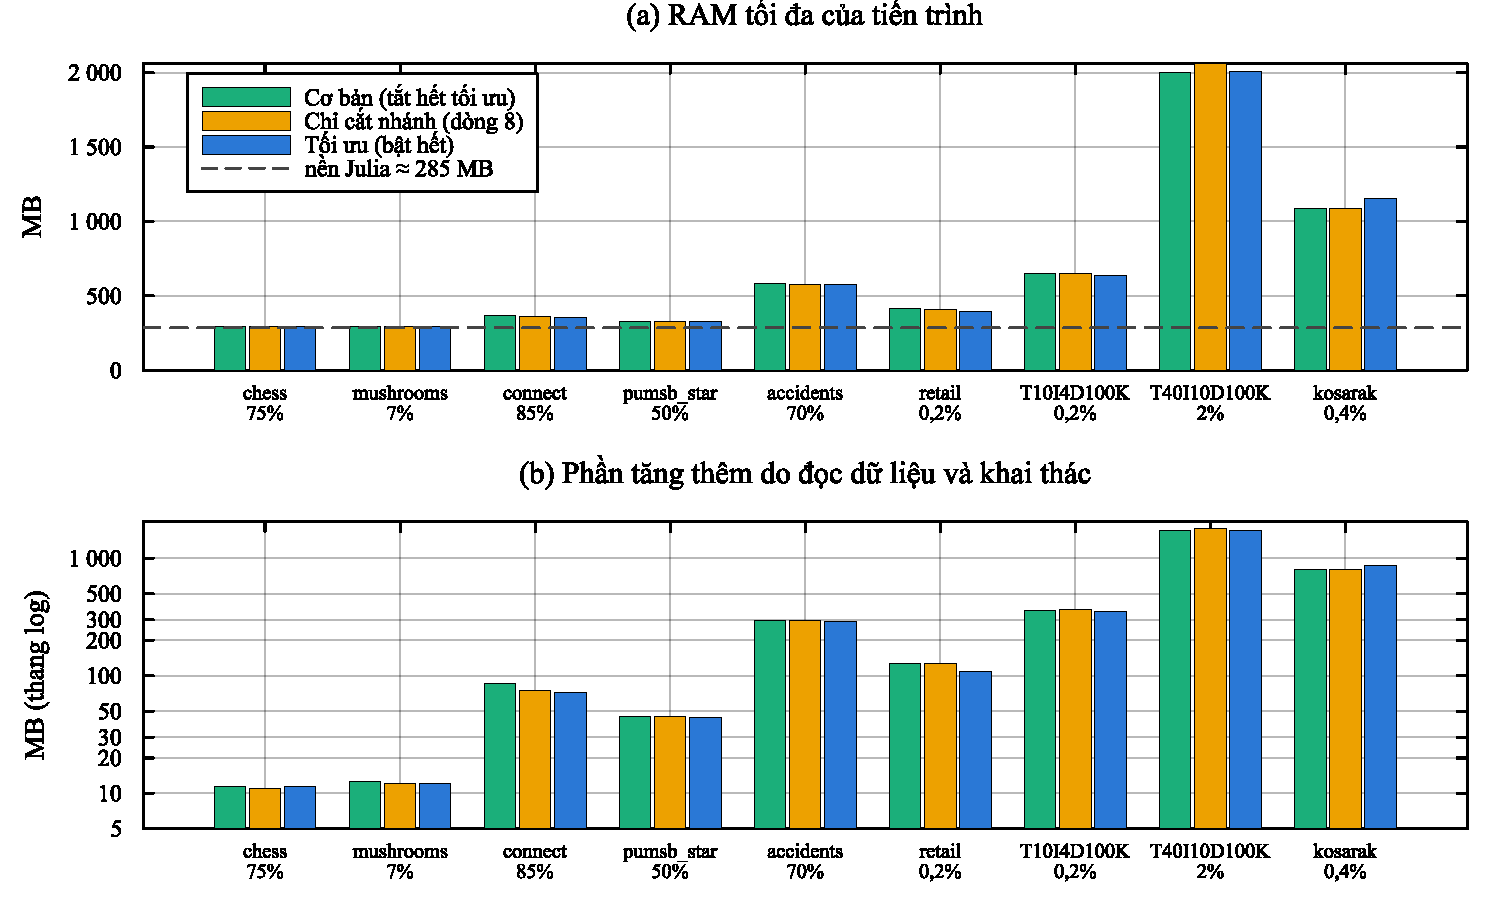
\includegraphics[width=\textwidth]{memory_basic_vs_optimized.pdf}
\caption{Bộ nhớ của ba biến thể tại minsup giữa lưới: (a) RAM tối đa của tiến trình (gồm khoảng 285\,MB nền của Julia),
(b) RAM tối đa tăng thêm so với mốc sau warm-up (\textit{incremental peak RSS}), thang log. Trung vị của 3 lần đo.}
\label{fig:memory}
\end{figure*}

\textbf{RAM tối đa.} Phần tăng thêm so với mốc sau warm-up đi từ khoảng 11\,MB trên chess đến khoảng 1{,}7\,GB trên
T40I10D100K và 0{,}8\,GB trên kosarak. Đây không phải bộ nhớ riêng của thuật toán mà gồm CSDL nạp vào bộ nhớ, FP-tree
gốc và các cây điều kiện đang mở trên đường đệ quy. T40I10D100K cần nhiều nhất vì FP-tree gốc gần như không nén được
(khoảng 3{,}26 triệu nút, $R_{\text{tree}}=89\%$) và giao dịch dài (trung bình 39{,}6 item).

\textbf{Bản tối ưu so với bản cơ bản.} Bản tối ưu giảm RAM tối đa trên connect (371 xuống 356\,MB), retail (414
xuống 399\,MB) và T10I4D100K (649 xuống 638\,MB), chênh lệch trên các CSDL còn lại khá nhỏ. Ngược lại, trên kosarak
RAM tối đa tăng từ 1\,089 lên 1\,153\,MB, khi tắt riêng FP-array thì còn 1\,101\,MB, cho thấy FP-array có thể làm
tăng chi phí bộ nhớ. Về thời gian khai thác, tỉ lệ bản cơ bản/bản tối ưu đi từ 0{,}98 trên accidents (bản cơ bản đo
được hơi nhanh hơn, trong phạm vi nhiễu) đến 1{,}32 trên mushrooms, tức bản tối ưu giảm khoảng 24\% thời gian khai
thác trên mushrooms. Phép thử loại bỏ (\textit{ablation}, Bảng~\ref{tab:ablation}, Phụ lục) tắt riêng từng tối ưu
và cho thấy lợi ích phụ thuộc CSDL:
\begin{itemize}
  \item Tắt \textbf{FP-array} làm thời gian khai thác tăng 28\% trên T40I10D100K và 18\% trên T10I4D100K. FP-array
        chỉ được dùng trên dữ liệu thưa (941 lần trên retail, 0 lần trên mọi CSDL dày) vì nó được tắt khi cây đủ dày,
        đúng như bài báo đề xuất~\cite{grahne2005}.
  \item \textbf{Cắt nhánh} và \textbf{kết thúc sớm} giảm số lời gọi đệ quy trên dữ liệu dày (mushrooms từ 15\,095
        xuống 8\,158, connect từ 13\,362 xuống 8\,212) và gần như không kích hoạt trên dữ liệu thưa.
  \item Tắt \textbf{CFI-tree rút gọn} làm thời gian khai thác tăng 13–16\% trên chess và mushrooms.
\end{itemize}
Các chênh lệch dưới khoảng 10\% được diễn giải thận trọng vì chỉ có ba lần đo. Chạy lại toàn bộ thực nghiệm bộ nhớ
trên một máy khác cho cùng tập kết quả ở cả 216 lần chạy, RAM tối đa lệch trung vị 0{,}9\% (Phụ lục~\ref{app:data}).

% ---------------------------------------------------------------------------
\subsection{Khả năng mở rộng}
\label{sec:scalability}

Nhóm dùng retail (88\,162 giao dịch) và tạo năm tập con lồng nhau gồm 10\%, 25\%, 50\%, 75\% và 100\% giao dịch (xáo
trộn một lần với seed cố định rồi lấy tiền tố), ở hai mức minsup tương đối 0{,}1\% và 0{,}05\%. Trong các tập con
này, số tập đóng gần ổn định theo kích thước: 7\,572–8\,394 ở 0{,}1\% và 18\,925–19\,579 ở 0{,}05\%.

\colfig{scalability_time.pdf}{Thời gian theo kích thước CSDL trên các tập con của retail.}{fig:sc-time}

Hình~\ref{fig:sc-time} (số liệu ở Bảng~\ref{tab:scalability} và Hình~\ref{fig:sc-ratio}, Phụ lục) cho thấy khi số
giao dịch tăng 10 lần, thời gian của nhóm tăng 10{,}5 lần ở minsup 0{,}1\% và 7{,}5 lần ở 0{,}05\%. Mô hình tuyến
tính $T(n)=an+b$ khớp tốt cho cả hai cài đặt ($R^2 \geq 0{,}97$), gợi ý xu hướng mở rộng gần tuyến tính trong phạm
vi retail và hai mức minsup khảo sát. Thời gian của SPMF chỉ tăng 3{,}1–3{,}5 lần, hệ số chặn $b$ của SPMF là
0{,}12–0{,}17\,s (22–25\% thời gian ở 100\%) còn của nhóm gần bằng 0. Hệ số chặn dương gợi ý SPMF có một thành phần
chi phí ít phụ thuộc kích thước dữ liệu, nhưng thực nghiệm này không xác định nguồn của chi phí đó. Hệ quả là nhóm
nhanh hơn SPMF trên các tập con nhỏ (0{,}071 so với 0{,}158\,s ở 10\%), gần tương đương ở 75\% với minsup 0{,}1\%
(1{,}09) và chậm hơn trên toàn bộ retail (0{,}75 so với 0{,}55\,s). Điều này nhất quán với Mục~\ref{sec:runtime}:
chi phí xử lý từng giao dịch của nhóm tăng theo khối lượng dữ liệu.

% ---------------------------------------------------------------------------
\subsection{Ảnh hưởng của độ dài giao dịch trung bình}
\label{sec:txlen}

Giao dịch dài có thể làm tăng độ sâu FP-tree, kích thước pattern base và số tổ hợp item cần khảo sát. Để kiểm
chứng, nhóm sinh sáu CSDL tổng hợp cùng 10\,000 giao dịch, miền 500 item, độ dài trung bình 5, 10, \ldots, 30. Giao
dịch của mức dài chứa giao dịch của mức ngắn, quy trình sinh nằm ở Phụ lục~\ref{app:data}. Vì miền item được giữ cố
định, khi độ dài tăng thì mật độ và mức đồng xuất hiện của item cũng thay đổi theo. Nhóm chạy ở hai mức minsup
0{,}5\% và 0{,}2\%.

\colfig{txlen_time.pdf}{Thời gian theo độ dài giao dịch trung bình (10\,000 giao dịch, 500 item).}{fig:tx-time}
\colfig{txlen_itemsets.pdf}{Số closed itemset theo độ dài giao dịch trung bình (10\,000 giao dịch, 500 item).}{fig:tx-items}

Hình~\ref{fig:tx-time} và~\ref{fig:tx-items} (số liệu ở Bảng~\ref{tab:txlen}, Phụ lục) cho thấy khi độ dài trung
bình tăng từ 5 lên 30, số tập đóng tăng khoảng 38 lần (470 lên 18\,038) ở minsup 0{,}5\% và 160 lần (914 lên
146\,134) ở 0{,}2\%, thời gian của nhóm tăng tương ứng khoảng 29 lần (0{,}017 lên 0{,}49\,s) và 98 lần (0{,}019 lên
1{,}89\,s). Thời gian và số tập đóng tăng nhanh trong khoảng độ dài 5–30, nhưng sáu điểm đo không đủ để khẳng định một
quy luật hàm mũ. Nhóm nhanh hơn hoặc gần tương đương SPMF ở mọi cấu hình khảo sát (tỉ lệ 0{,}34 ở độ dài 5,
0{,}76–0{,}82 ở độ dài 30). Tại minsup 0{,}2\% và độ dài 20, 25, tỉ lệ là 0{,}93 và 0{,}98, tức gần tương đương. Nhìn
chung lợi thế của nhóm thu hẹp khi giao dịch dài ra.

% ---------------------------------------------------------------------------
\subsection{Phân tích độ phức tạp}
\label{sec:complexity}

Gọi $n$ là số giao dịch, $L=\sum_i |T_i|$ là tổng số lượt item ban đầu, $m$ là số item phổ biến và $k_i$ là độ dài
giao dịch thứ $i$ sau khi lọc item không phổ biến. Bảng~\ref{tab:complexity} tóm tắt chi phí từng thành phần với giả
định đếm, tra thứ tự và chèn nút có chi phí trung bình $O(1)$. Nhóm không đưa ra một cận Big-O duy nhất cho toàn bộ
FPClose, vì chi phí khai thác phụ thuộc cấu trúc dữ liệu và không chỉ phụ thuộc kích thước đầu vào hay đầu ra.

\begin{table}[!htb]
\caption{Chi phí các thành phần của FPClose và liên hệ với thực nghiệm}
\label{tab:complexity}
\centering
\footnotesize\setlength{\tabcolsep}{3pt}
\begin{tabular}{@{}>{\raggedright\arraybackslash}p{0.19\columnwidth}>{\raggedright\arraybackslash}p{0.48\columnwidth}>{\raggedright\arraybackslash}p{0.27\columnwidth}@{}}
\hline
Thành phần & Chi phí & Liên hệ thực nghiệm \\
\hline
FP-tree gốc & $O(L + m\log m + \sum_i k_i\log(k_i+1))$ thời gian, tối đa $\sum_i k_i$ nút không tính gốc &
Khả năng mở rộng, bước xử lý giao dịch \\
FP-array & $O(m^2)$ bộ nhớ (nửa tam giác dưới), $O(m^2 + \sum_i k_i^2)$ thời gian nếu khởi tạo cả mảng và đếm mọi
cặp, chỉ tính khi cây được coi là thưa & Đánh đổi thời gian và bộ nhớ (kosarak) \\
Khai thác đệ quy & Phụ thuộc số trạng thái được duyệt, kích thước pattern base và cây điều kiện. Số tập đóng tối đa
$O(2^m)$ & minsup, kích thước đầu ra, độ dài giao dịch \\
Kiểm tra đóng & Phụ thuộc số nút ứng viên của CFI-tree được duyệt và chi phí kiểm tra bao hàm & Cắt nhánh, CFI-tree
rút gọn \\
Bộ nhớ & CSDL $O(L)$, cây gốc, các cây điều kiện, FP-array và CFI-tree còn sống trên đường đệ quy, stack & RAM tối đa
\\
\hline
\end{tabular}
\end{table}

% ---------------------------------------------------------------------------
\subsection{Đánh giá chung và hướng tối ưu}
\label{sec:discussion}

\textbf{Điểm mạnh và điểm yếu.} Cài đặt của nhóm khớp SPMF trên cả 56 cấu hình closed itemset và có lợi thế trên các
CSDL dày có nhiều tập đóng như chess, mushrooms, connect ở minsup thấp nhất. Tuy nhiên, hiệu năng không đồng nhất trên
mọi CSDL: nhóm chậm hơn trên accidents, pumsb\_star, kosarak và T10I4D100K, bước đọc dữ liệu là một điểm nghẽn tiềm
năng trên các CSDL lớn (khoảng 1{,}1\,s trên accidents và kosarak), và các tối ưu có thể làm tăng RAM tối đa như
FP-array trên kosarak. Lợi ích của các tối ưu phụ thuộc CSDL và chỉ số được đo.

\textbf{Giới hạn.} Kết quả chỉ phản ánh các cấu hình khảo sát. Ba lần đo mỗi cấu hình, cách warm-up khác nhau giữa
Julia và JVM, và việc khảo sát khả năng mở rộng chỉ trên retail giới hạn khả năng suy rộng.

\textbf{Hướng tối ưu tiếp theo.}
\begin{enumerate}
  \item \textbf{Đọc dữ liệu nhanh hơn.} Bộ đọc hiện tại tách từng dòng thành chuỗi và cấp phát một vector cho mỗi
        giao dịch. Có thể phân tích số nguyên trực tiếp từ bộ đệm byte và lưu CSDL thành một mảng phẳng
        (\texttt{Vector\{Int32\}}) kèm mảng vị trí bắt đầu của từng giao dịch, để giảm tạo chuỗi và cấp phát.
  \item \textbf{Giảm cấp phát khi dựng cây.} Thay các nút là đối tượng riêng bằng cấu trúc mảng (\textit{struct of
        arrays}: mảng item, count, cha, node-link dạng \texttt{Int32}) và tái sử dụng vùng nhớ theo vòng đời của
        từng tầng đệ quy. Cần đo lại bộ nhớ cấp phát và RAM tối đa khi triển khai.
  \item \textbf{FP-array thích nghi.} Điều chỉnh quyết định bật hay tắt FP-array cho từng cây điều kiện theo số item,
        tỉ lệ nén thực đo và ngân sách bộ nhớ, thay cho các ngưỡng cố định hiện tại (\texttt{dense\_ratio},
        \texttt{skip\_items}). Đây là hướng cải tiến cho cơ chế hiện có, chưa được triển khai và kiểm chứng.
\end{enumerate}
   % Chương 2: Thực nghiệm và đánh giá
% Chương 3: Ứng dụng thực tế. KHUNG: các mục theo đề (https://hcmus-cs-ta.github.io/lab-book/data-mining/projects/itemset/),
% thành viên phụ trách Chương 3 thay các \todo{...} bằng nội dung. Mọi kết quả phải chạy bằng chính cài đặt của nhóm;
% phần biến đổi dữ liệu thành giao dịch cài cùng mã chuẩn bị dữ liệu trong demo notebook.

\section{\texorpdfstring{Ứng dụng thực tế}{CHƯƠNG 3: ỨNG DỤNG THỰC TẾ}}
\label{sec:applications}

Chương này áp dụng cài đặt FPClose của nhóm vào hai bài toán trên dữ liệu thực, mỗi bài toán có một cách biến đổi dữ
liệu ban đầu thành giao dịch riêng. Ở Ứng dụng 1 (Mục~\ref{sec:app1}), mỗi hóa đơn của một cửa hàng bán lẻ trực tuyến
là một giao dịch và mỗi mã sản phẩm (StockCode) là một item; các tập phổ biến được dùng để sinh luật kết hợp. Ở Ứng
dụng 2 (Mục~\ref{sec:app2}), mỗi ảnh là một giao dịch và mỗi từ thị giác (\textit{visual word}, cụm đặc trưng cục bộ
của ảnh) là một item. Trong cả hai ứng dụng, các thư viện khác chỉ được dùng để tạo giao dịch định dạng SPMF và trình
bày kết quả; mọi tập phổ biến đóng đều được khai thác bằng FPClose của nhóm, không dùng thư viện khai thác tập phổ biến
nào khác.

\subsection{Ứng dụng 1}
\label{sec:app1}
\subsubsection{Bài toán và dữ liệu}
Ứng dụng tìm các nhóm sản phẩm thường được mua cùng nhau trong một cửa hàng bán lẻ trực tuyến, sinh luật kết hợp
$A \rightarrow B$ từ các nhóm đó và diễn giải mười luật có lift cao nhất. Dữ liệu là UCI Online Retail~\cite{uci_retail}
(giấy phép CC BY 4.0), gồm 541\,909 dòng của một cửa hàng trực tuyến tại Vương quốc Anh trong giai đoạn 12/2010--12/2011.
Mỗi dòng là một sản phẩm trong một hóa đơn, với mã hóa đơn (InvoiceNo), mã sản phẩm (StockCode), mô tả, số lượng, thời
điểm, đơn giá, mã khách hàng (CustomerID) và quốc gia. File gốc được kiểm tra mã băm SHA-256 trước khi xử lý để mọi lần
chạy dùng cùng một phiên bản dữ liệu. Toàn bộ quy trình nằm trong \path{notebooks/application_01.ipynb} và
\path{applications/application_01/market_basket.py}.

\subsubsection{Biến đổi thành giao dịch}
Mỗi giao dịch là một hóa đơn và mỗi item là một StockCode. Các bước làm sạch được áp dụng theo thứ tự cố định, bước sau
trên kết quả của bước trước: (1) bỏ dòng thiếu InvoiceNo hoặc StockCode (không có dòng nào); (2) bỏ 9\,288 dòng của
3\,836 hóa đơn hủy (InvoiceNo bắt đầu bằng ``C''); (3) bỏ 1\,336 dòng có số lượng không dương; (4) bỏ 1\,181 dòng có
đơn giá không dương; (5) bỏ dòng thiếu mô tả (không còn dòng nào, vì cả 1\,454 dòng thiếu mô tả đã bị loại ở các bước
trước); (6) bỏ 2\,379 dòng thuộc 32 StockCode lệch khỏi mẫu mã sản phẩm thông thường (năm chữ số, có thể kèm tối đa
hai chữ cái). Các mã này gồm hai loại. Loại thứ nhất là mã thật sự không phải hàng hóa: phí vận chuyển (POST, DOT, C2),
điều chỉnh kế toán và phí (M, D, B, BANK CHARGES, AMAZONFEE, CRUK), hàng mẫu (S) và phiếu quà tặng (GIFT\_*); chúng
được bỏ vì không biểu diễn sản phẩm được mua. Loại thứ hai là hàng hóa mang mã đặc biệt: mã của kênh bán riêng (DCGS*,
một số có mô tả như túi tiệc, vòng cổ cho chó) và PADS (miếng lót đệm). Nhóm bỏ cả loại này để giữ item là mã sản phẩm
thông thường; quyết định này không ảnh hưởng tới kết quả, vì mỗi mã chỉ có trong không quá 13 hóa đơn, ít hơn ngưỡng
thấp nhất được khảo sát (40 hóa đơn), nên không thể thuộc tập phổ biến nào, và việc bỏ một mã không làm đổi support tuyệt
đối của các itemset không chứa mã đó. Sau làm sạch còn 527\,725 dòng (97,4\%).

Trong 541\,909 dòng gốc, 135\,080 dòng (24,9\%) thiếu CustomerID; sau làm sạch còn 131\,388 trong 527\,725 dòng (cũng
24,9\%). Các dòng này được giữ lại, vì giao dịch được xác định theo InvoiceNo chứ không theo khách hàng. Mỗi giao dịch là \emph{tập} các StockCode phân biệt của một hóa đơn: số lượng không được dùng và 10\,471 dòng trùng
mã trong cùng hóa đơn được gộp, đúng với dạng đầu vào của FPClose. Hóa đơn chỉ có một sản phẩm vẫn được giữ (7,59\% số
giao dịch). Kết quả là 19\,773 giao dịch trên 3\,791 item; con số này nhỏ hơn 22\,064 hóa đơn không bị hủy vì 2\,291
hóa đơn chỉ gồm các dòng đã bị loại. Mỗi StockCode được ánh xạ sang một số nguyên và giao dịch được ghi theo định dạng
SPMF, kèm bảng ánh xạ để dịch kết quả về tên sản phẩm.

Độ dài giỏ hàng có trung bình 26,2, trung vị 15 và lớn nhất 1\,106 sản phẩm. Phân bố lệch phải: 236 hóa đơn (1,2\%) có
từ 200 sản phẩm và 49 hóa đơn (0,25\%) có từ 500 sản phẩm trở lên. Các hóa đơn rất dài này nhiều khả năng là đơn bán
sỉ, nhưng dữ liệu không ghi loại khách hàng nên chúng được giữ lại và ảnh hưởng của chúng được đánh giá riêng. Mật độ
(độ dài trung bình chia cho số item) là 0,69\%; theo Bảng~\ref{tab:datasets}, giá trị này nằm trong khoảng mật độ của
các CSDL thưa ở Chương~2 (0,020--4,204\%), thấp hơn T10I4D100K (1,161\%) nhưng cao hơn retail (0,063\%) và kosarak
(0,020\%).

\begin{table}[!t]
\centering
\caption{Top-10 luật theo lift ở minsup 1\%, minconf 0,6. Mọi sản phẩm thuộc dòng que cắm cây gia vị HERB MARKER,
ghi theo tên cây. Support tính theo \% số giao dịch.}
\label{tab:app1-top10}
\footnotesize\setlength{\tabcolsep}{4pt}
\begin{tabular}{rllrrr}\hline
\# & Vế trái & Vế phải & Supp. (\%) & Conf. & Lift\\\hline
1 & Thyme & Rosemary + Parsley & 1{,}03 & 0{,}86 & 78{,}8\\
2 & Rosemary + Parsley & Thyme & 1{,}03 & 0{,}94 & 78{,}8\\
3 & Thyme + Parsley & Rosemary & 1{,}03 & 0{,}95 & 78{,}5\\
4 & Rosemary & Thyme + Parsley & 1{,}03 & 0{,}85 & 78{,}5\\
5 & Thyme + Basil & Rosemary & 1{,}01 & 0{,}95 & 78{,}5\\
6 & Rosemary & Thyme + Basil & 1{,}01 & 0{,}83 & 78{,}5\\
7 & Rosemary + Basil & Thyme & 1{,}01 & 0{,}93 & 78{,}0\\
8 & Thyme & Rosemary + Basil & 1{,}01 & 0{,}84 & 78{,}0\\
9 & Thyme & Rosemary & 1{,}12 & 0{,}93 & 76{,}8\\
10 & Rosemary & Thyme & 1{,}12 & 0{,}92 & 76{,}8\\
\hline
\end{tabular}
\end{table}

\begin{table*}[!t]
\centering
\caption{Top-10 luật đa dạng ở minsup 1\%, minconf 0,6: các luật không có sản phẩm chung, chọn theo thứ tự xếp hạng của
toàn bộ 574 luật. Hạng là vị trí trong toàn bộ luật. Tên sản phẩm rút gọn thành ``dòng sản phẩm: biến thể'', phần biến
thể giữ nguyên tiếng Anh (tên đầy đủ và StockCode có trong \texttt{top10\_rules\_diverse.csv}). Cột cuối là lift khi bỏ 236
hóa đơn có từ 200 sản phẩm trở lên; ``không đạt'' nghĩa là luật không còn đạt hai ngưỡng.}
\label{tab:app1-diverse}
\footnotesize
\begin{tabular}{rlrrrr}\hline
Hạng & Luật & Supp. (\%) & Conf. & Lift & Lift khi bỏ hóa đơn $\geq 200$ sản phẩm\\\hline
1 & Herb Marker: Thyme $\rightarrow$ Rosemary + Parsley & 1{,}03 & 0{,}86 & 78{,}8 & không đạt\\
31 & Herb Marker: Mint $\rightarrow$ Basil & 1{,}05 & 0{,}87 & 70{,}8 & không đạt\\
33 & Regency đĩa trà: Pink $\rightarrow$ Roses + Green & 1{,}29 & 0{,}84 & 51{,}8 & 63{,}4\\
40 & Trang trí gỗ: Tree $\rightarrow$ Stocking & 1{,}11 & 0{,}75 & 46{,}3 & không đạt\\
42 & Regency: Sugar Bowl Green $\rightarrow$ Milk Jug Pink & 1{,}23 & 0{,}75 & 45{,}4 & 52{,}4\\
44 & Poppy's Playhouse: Livingroom $\rightarrow$ Bedroom + Kitchen & 1{,}13 & 0{,}68 & 43{,}1 & 49{,}4\\
46 & Hũ mứt: Green Lid $\rightarrow$ Pink Lid & 1{,}15 & 0{,}74 & 42{,}9 & không đạt\\
50 & Cốc chấm bi: Pink $\rightarrow$ Blue & 1{,}05 & 0{,}68 & 41{,}2 & 46{,}6\\
52 & Dao nĩa trẻ em: Dolly Girl $\rightarrow$ Spaceboy & 1{,}15 & 0{,}76 & 41{,}0 & 43{,}6\\
61 & Bát chấm bi: Blue $\rightarrow$ Pink & 1{,}05 & 0{,}65 & 38{,}4 & 42{,}9\\
\hline
\end{tabular}
\end{table*}

\subsubsection{Khai thác và chọn tham số}
Mọi kết quả được sinh bằng \texttt{demo.jl} của nhóm theo ba bước: FPClose khai thác các tập phổ biến đóng, bước khôi
phục suy ra mọi tập phổ biến theo \eqref{eq:recovery}, và bước sinh luật tách mỗi tập phổ biến $Z = A \cup B$
(Mục~\ref{sec:basic}). Một luật được giữ khi $\mathrm{support}(A \cup B) \geq \mathit{minsup}$, nên $A$, tập con của
$Z$, cũng phổ biến, và khi confidence đạt minconf; support, confidence và lift được tính theo các công thức ở
Mục~\ref{sec:basic}.

\begin{figure}[!t]
\centering
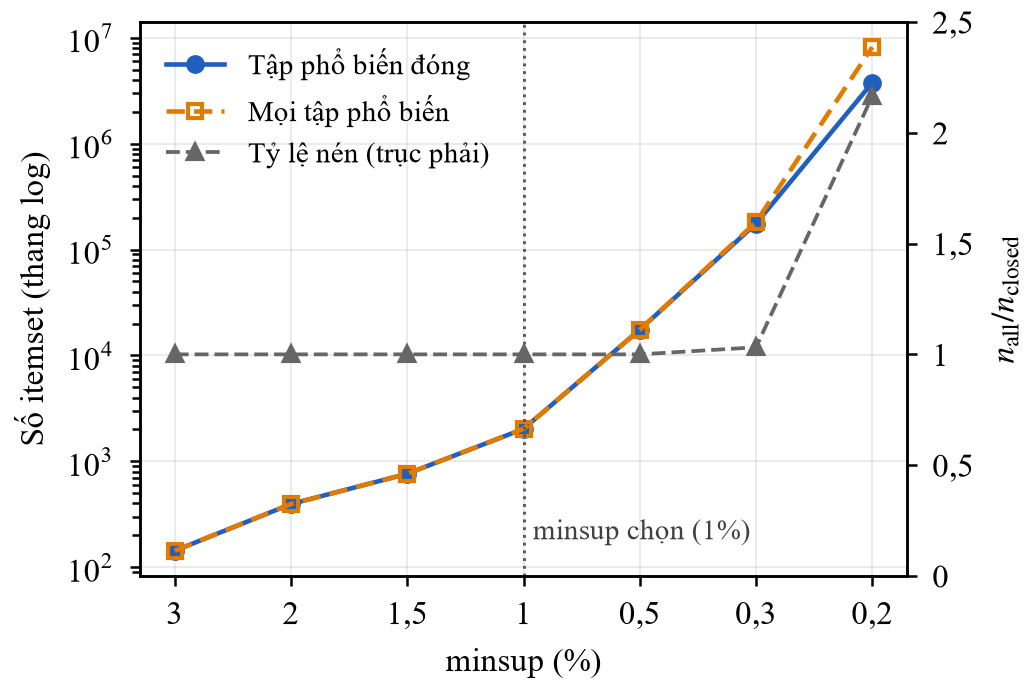
\includegraphics[width=\columnwidth]{figures/app1_minsup_survey.png}
\caption{Số tập phổ biến đóng, số mọi tập phổ biến (trục trái, thang log) và tỷ lệ nén
$n_{\mathrm{all}}/n_{\mathrm{closed}}$ (trục phải) theo minsup trên UCI Online Retail. Hai đường số tập trùng nhau từ
3\% đến 0,5\%; vạch chấm đánh dấu minsup được chọn.}
\label{fig:app1-minsup}
\end{figure}

Vì sản phẩm phổ biến nhất chỉ có support 11,5\%, minsup được khảo sát trong khoảng 3\% đến 0,2\%
(Hình~\ref{fig:app1-minsup}). Từ 3\% xuống 0,5\%, số tập đóng tăng từ 143 lên 17\,498 và luôn bằng số tập phổ biến:
trên dữ liệu thưa này, hầu như không có tập nào mà mọi hóa đơn chứa nó đều chứa thêm một sản phẩm chung khác. Tỷ lệ nén
chỉ vượt 1 ở 0,3\% (1,03) và đạt 2,16 ở 0,2\%. Từ 0,3\% xuống 0,2\%, số tập đóng tăng khoảng 21 lần, từ 176\,102 lên
3\,771\,107. Để kiểm tra ảnh hưởng của hóa đơn rất dài, nhóm chạy lại sau khi bỏ hóa đơn theo hai ngưỡng độ dài. Ngưỡng
500 sản phẩm chỉ bỏ 49 hóa đơn (0,25\% số giao dịch), nên dùng để hỏi liệu một nhóm rất nhỏ có đủ gây ra bước nhảy hay
không: số tập đóng ở 0,2\% giảm còn 424\,270, tức khoảng 88,7\%. Số tập đóng ở mức này vì vậy rất nhạy với nhóm hóa
đơn cực dài, dù kết quả không cho thấy mọi tập bị mất chỉ nằm trong các hóa đơn đó, vì việc bỏ hóa đơn cũng làm thay
đổi tập nào là tập đóng. Ngưỡng 200 sản phẩm bỏ 236 hóa đơn (1,2\%) và làm số tập đóng ở 1\% giảm từ 2\,026 xuống
1\,267, so với 1\,668 khi dùng ngưỡng 500; vì đây là phép thử chặt hơn trong hai ngưỡng, nó được dùng để kiểm tra độ ổn
định của luật trong phần kết quả luật bên dưới. Nhóm chọn minsup 1\%
để sinh luật, vì mỗi mẫu dựa trên ít nhất 198 hóa đơn và số tập phổ biến vừa phải (2\,026, trong đó 1\,197 tập có từ hai
sản phẩm); các mức dưới 1\% chỉ dùng để khảo sát. Ngưỡng confidence được đặt là $\mathit{minconf} = 0{,}6$.

Ở minsup 1\% (198 giao dịch), FPClose tìm được 2\,026 tập đóng, đúng bằng số tập phổ biến sau khôi phục, và bước sinh
luật cho 574 luật. Như vậy, ở cấu hình này biểu diễn tập đóng \emph{không đem lại lợi ích nén} (tỷ lệ nén 1,0); lợi ích
đó chỉ xuất hiện từ minsup 0,3\% trở xuống. Quy trình vẫn đáp ứng mục tiêu ứng dụng, vì luật được sinh từ mọi tập phổ
biến khôi phục đầy đủ từ tập đóng. Thời gian khai thác khoảng 0,4--0,5\,s, khoảng 3\,s nếu tính cả thời gian khởi động Julia. Để kiểm
tra độc lập với FPClose, support, confidence và lift của cả 574 luật được tính lại bằng phép đếm trực tiếp trên tập giao
dịch; 574/574 luật khớp, với sai số dưới $10^{-9}$. Phép kiểm này xác nhận các luật được sinh ra là đúng, nhưng không
chứng minh tập luật là đầy đủ; tính đầy đủ dựa trên việc tập phổ biến đã được đối chiếu với SPMF
(Mục~\ref{sec:correctness}) và bộ kiểm thử của bước sinh luật (Mục~\ref{sec:tests}).

\subsubsection{Kết quả luật}
Bảng~\ref{tab:app1-top10} trình bày mười luật có lift cao nhất. Cả mười luật đều thuộc bộ que cắm cây gia vị HERB MARKER,
với lift từ 76,8 đến 78,8 và confidence từ 0,83 đến 0,95: trong các hóa đơn chứa vế trái, tỷ lệ chứa vế phải cao gấp gần
80 lần tỷ lệ chung. Support chỉ từ 1,01\% đến 1,12\% (200--221 hóa đơn), sát ngưỡng minsup. Các luật đi theo cặp đối
xứng có cùng lift, vì $\mathrm{lift}(A \rightarrow B) = \mathrm{lift}(B \rightarrow A)$; tám luật đầu được tách từ hai
tập ba sản phẩm $\{$Thyme, Rosemary, Parsley$\}$ và $\{$Thyme, Rosemary, Basil$\}$. Khi bỏ 236 hóa đơn có từ 200 sản
phẩm trở lên (1,2\% số giao dịch), số luật ở minsup 1\% giảm từ 574 xuống 296, và 8/10 luật của
Bảng~\ref{tab:app1-top10} không còn đạt ngưỡng; chỉ cặp Thyme $\leftrightarrow$ Rosemary còn lại, với lift tăng từ 76,8
lên 85,0.

Vì top-10 theo lift bị một dòng sản phẩm chi phối, nhóm lập thêm Bảng~\ref{tab:app1-diverse} để bổ sung, không thay thế
Bảng~\ref{tab:app1-top10}. Các luật được duyệt theo đúng thứ tự xếp hạng của toàn bộ 574 luật, và một luật chỉ được nhận
khi không có sản phẩm nào của nó đã xuất hiện trong các luật đã nhận; cách lọc này chỉ chọn lại trong các luật FPClose đã
sinh ra. Mười luật trải trên nhiều dòng sản phẩm, với lift từ 38,4 đến 78,8 và confidence từ 0,65 đến 0,87. Vì phép lọc
chỉ bảo đảm không trùng mã sản phẩm, một số dòng xuất hiện ở hai luật (như HERB MARKER và Regency). Khi bỏ hóa đơn từ 200 sản
phẩm, sáu luật vẫn đạt ngưỡng và có lift tăng, còn bốn luật (hai luật HERB MARKER, đồ trang trí gỗ và hũ mứt) không còn
đạt. Ở minsup 2\%, chỉ còn 30 luật (30/30 khớp phép đếm trực tiếp), và không luật nào của Bảng~\ref{tab:app1-diverse} đạt
ngưỡng này, vì support của chúng chỉ từ 1,03\% đến 1,29\%. Luật đứng đầu ở 2\% thuộc bộ tách trà Regency, với support
2,74\% và lift 18,2: các luật ở ngưỡng cao hơn thuộc các bộ sưu tập bán chạy hơn và có lift thấp hơn, nhưng vẫn nối các
biến thể của cùng một bộ sưu tập.

\subsubsection{Ý nghĩa kinh doanh và giới hạn}
Các luật nổi bật chủ yếu nối các biến thể khác màu hoặc khác mẫu của cùng một bộ sưu tập: que cắm theo loại cây, đĩa trà
và bộ bát đường, bình sữa Regency theo màu, các phòng của bộ đồ chơi Poppy's Playhouse, cốc và bát chấm bi, dao nĩa trẻ
em theo mẫu. Từ đó nhóm nêu một số \emph{đề xuất chưa được kiểm chứng}. Thứ nhất, khi khách chọn một biến thể, hệ thống
có thể gợi ý các biến thể còn lại của bộ sưu tập; nên ưu tiên thử với sáu luật của Bảng~\ref{tab:app1-diverse} vẫn đạt
ngưỡng khi bỏ hóa đơn rất dài. Thứ hai, các mẫu chỉ đạt ngưỡng nhờ hóa đơn rất dài (trọn bộ HERB MARKER, đồ trang trí gỗ,
hũ mứt) phù hợp hơn với gói sản phẩm cho đơn hàng số lượng lớn. Thứ ba, luật có lift cao nhưng support khoảng 1\% hợp với
gợi ý nhắm đúng khách hàng, còn luật có support cao hơn như ở minsup 2\% hợp với khuyến mãi diện rộng. Hiệu quả của các
đề xuất này cần được đo bằng thử nghiệm A/B trước khi áp dụng.

Kết quả có các giới hạn sau. Luật chỉ phản ánh sự đồng xuất hiện trong cùng hóa đơn, không phải quan hệ nhân quả hay
thứ tự mua. Dữ liệu không ghi loại khách hàng, nên độ dài hóa đơn chỉ là dấu hiệu gián tiếp của đơn bán sỉ. Mỗi biến thể
là một StockCode riêng, nên luật chủ yếu nối các biến thể cùng dòng và ít cho thấy quan hệ giữa các dòng sản phẩm khác
nhau. Số lượng, đơn giá và thời gian mua chưa được dùng, nên luật chưa phản ánh doanh thu hay mùa vụ; dữ liệu cũng chỉ
thuộc một cửa hàng tại Vương quốc Anh trong giai đoạn 2010--2011.

\subsection{Ứng dụng 2: Khai thác mẫu trực quan trên ảnh}
\label{sec:app2}

\subsubsection{Bài toán và dữ liệu}
Ứng dụng tìm các tổ hợp từ thị giác (\textit{visual words}) phổ biến trong từng lớp ảnh, khảo sát chúng mô tả
vật thể hay vùng nền, và thử sử dụng chúng làm đặc trưng phân loại. Nhóm dùng Caltech-101~\cite{caltech101},
chọn năm lớp airplanes, Motorbikes, Faces\_easy, watch và Leopards. Mỗi lớp lấy 200 ảnh, chia phân tầng thành
140 ảnh train và 60 ảnh test, tổng cộng 700/300 ảnh; seed bằng 42. Các lớp có hình dạng và kết cấu khác nhau,
thuận tiện cho việc quan sát mẫu. Đây là nghiên cứu trường hợp trên năm lớp, không phải đánh giá toàn bộ
Caltech-101. Không dùng Faces để tránh trùng với Faces\_easy, hoặc lớp nền BACKGROUND\_Google.

\subsubsection{Biến đổi ảnh thành giao dịch}
Ảnh được chuyển sang mức xám, giữ tỉ lệ khi resize cạnh dài về 400 pixel. SIFT~\cite{lowe2004} được cấu hình
\texttt{nfeatures=500}; lưu descriptor cùng tọa độ keypoint để đối chiếu mẫu với ảnh. Bộ ảnh cho 449\,891 keypoint,
trong đó 315\,643 thuộc train. Nhóm lấy khoảng 150\,000 descriptor train, giới hạn tối đa 221 descriptor mỗi ảnh
để giảm sự áp đảo của ảnh nhiều keypoint, rồi học codebook bằng MiniBatchKMeans với $k\in\{100,300\}$,
\texttt{n\_init=3}, \texttt{batch\_size=4096}, seed 42. Mỗi descriptor được gán vào tâm gần nhất theo khoảng
cách Euclid. Codebook chỉ học trên train; test dùng lại các tâm đã học.
SIFT và k-means phụ thuộc nền tảng: cùng mã nguồn, seed và phiên bản thư viện, chạy trên Colab (Linux) cho cùng
vị trí keypoint với máy Windows dùng cho báo cáo nhưng descriptor khác (chỉ 28,8\% keypoint trùng descriptor); với
cùng đầu vào, codebook $k=100$ trùng từng byte còn $k=300$ khác (ARI 0,33, inertia lệch +0,07\%). Vì vậy notebook dùng lại đặc trưng SIFT, codebook
và phép gán từ đã lưu của lần chạy chính (kiểm tra SHA-256) để tái lập đúng số liệu; SIFT và k-means vẫn được tính
lại trên máy đang chạy trong các ô kiểm chứng để so với bản đã lưu.

Gọi $n_i(w)$ là số keypoint của ảnh $i$ được gán vào từ $w\in\{0,\ldots,k-1\}$. Giao dịch của ảnh là
\begin{equation}
T_i=\{w+1\mid n_i(w)\geq\tau,\ w\notin S\},\qquad \tau=3,
\label{eq:app2-transaction}
\end{equation}
trong đó $S$ gồm các từ có mặt, sau ngưỡng $\tau$, trong hơn 80\% ảnh train. Item được cộng 1 để có mã dương,
sắp tăng và không lặp khi xuất định dạng SPMF. Mỗi giao dịch ghi nhận sự đồng xuất hiện trên toàn ảnh,
không khẳng định các từ kề nhau hay tạo thành một bộ phận vật thể.

Ngưỡng $\tau$ được chọn theo quy tắc định trước: với stop word 80\%, lấy $\tau$ lớn nhất trong $\{1,2,3\}$
có accuracy CV 5-fold trên train không thấp hơn mức tốt nhất quá 0,01. Mô hình dùng để chọn là Logistic
Regression trên vector hiện diện từng item, không phải vector mẫu khai thác. Cả hai codebook chọn $\tau=3$.
Đây là chỉ báo nội bộ: codebook và stop word được học trên toàn bộ train trước khi chia fold, nên chưa phải
CV của toàn pipeline. Tập test cuối không tham gia lựa chọn này.

Không có giao dịch rỗng ở cấu hình đã chọn. Độ dài trung bình trên train là 57,0 item với $k=100$ và 58,1
với $k=300$; riêng airplanes chỉ đạt 37,7 và 31,5. Stop word loại tương ứng một và không từ, do đó tác động
lọc trong cấu hình này rất nhỏ. Các bước trên được cài trong notebook và các script phụ trợ; OpenCV và
scikit-learn phục vụ trích đặc trưng, gom cụm và đánh giá, còn khai thác tập phổ biến dùng cài đặt của nhóm.

\begin{figure*}[!t]
\centering
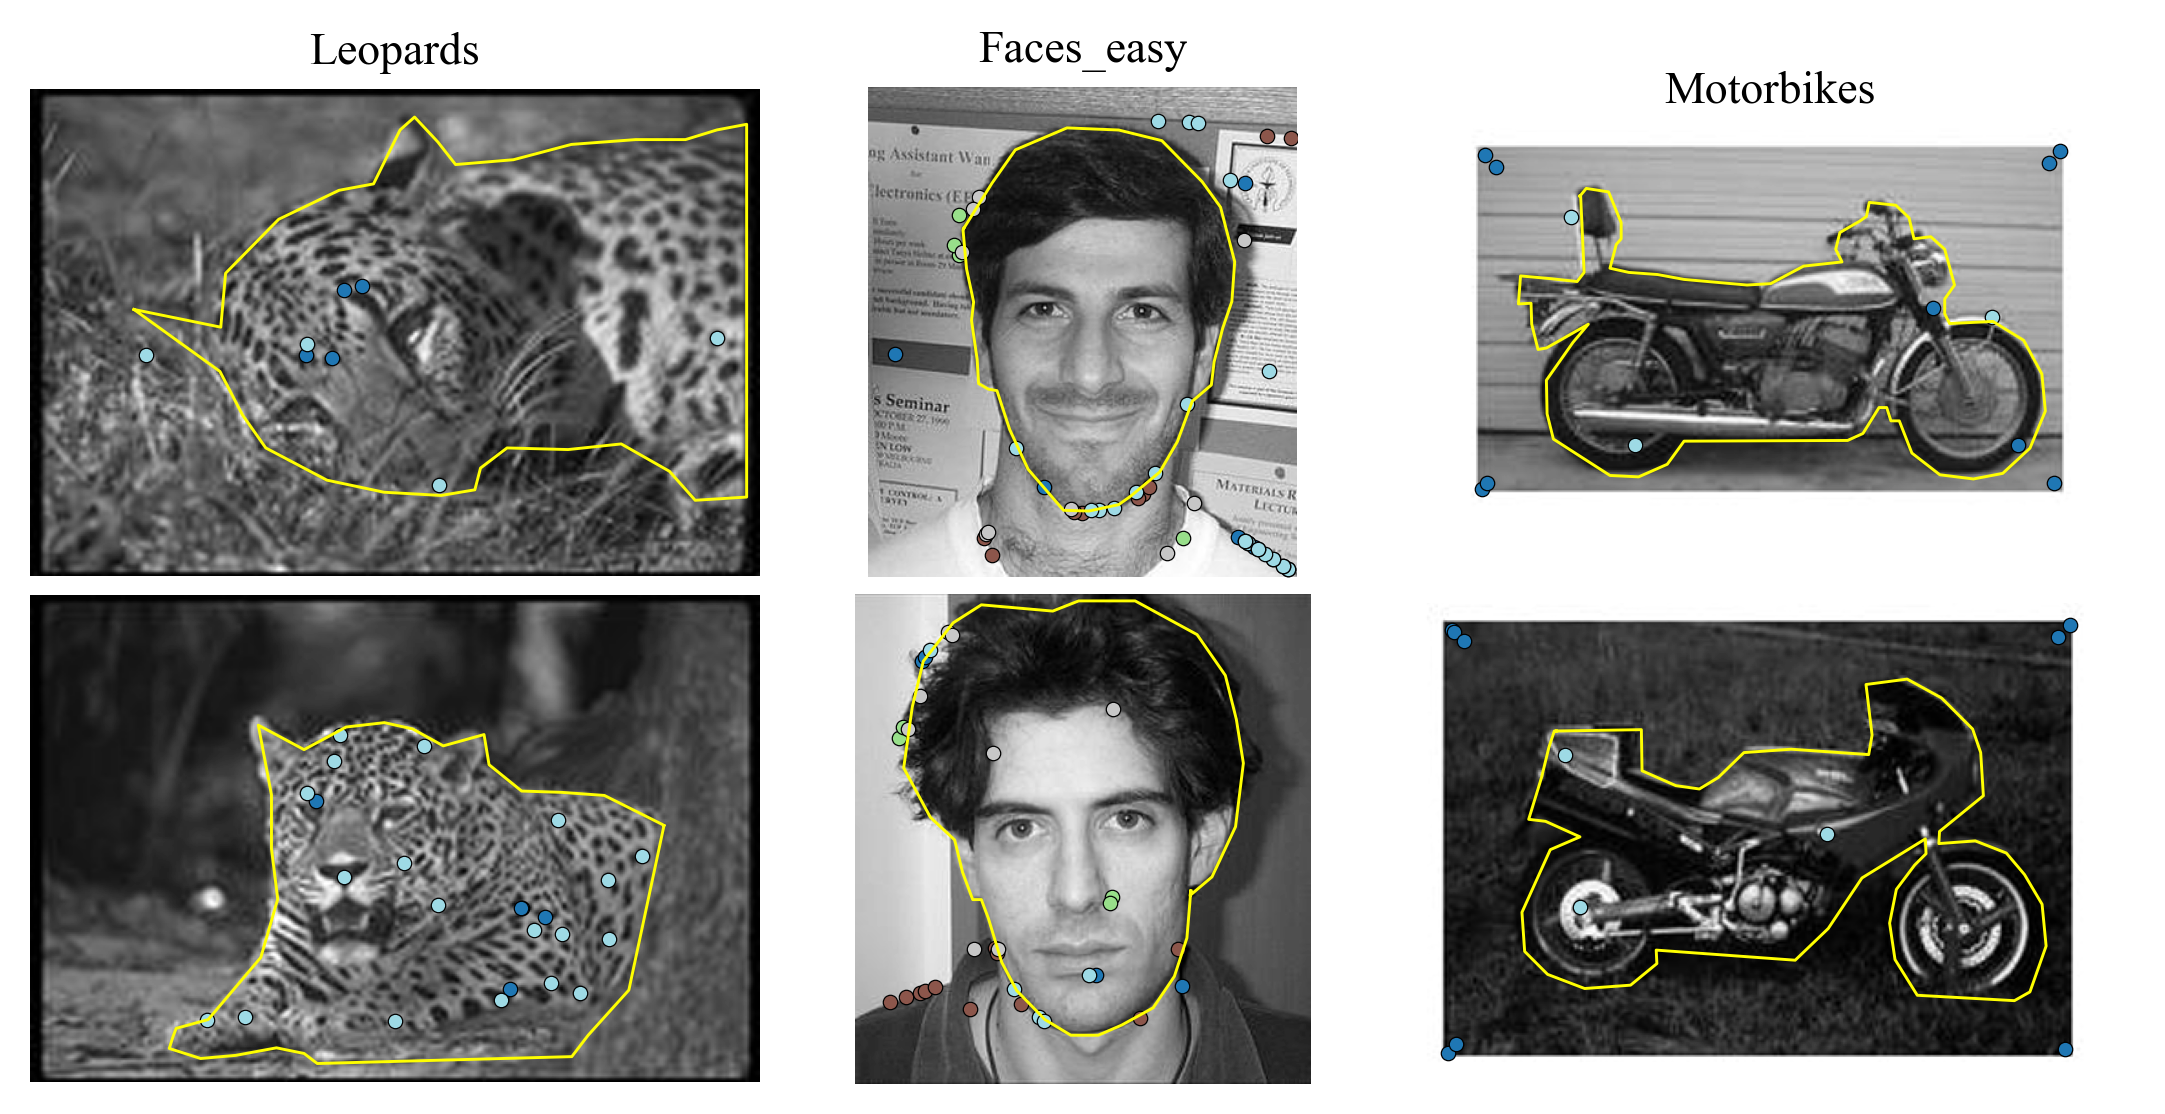
\includegraphics[width=0.92\textwidth]{figures/app2_patterns.png}
\caption{Mẫu top-1 tại $k=300$ của ba lớp Leopards, Faces\_easy và Motorbikes, mỗi lớp hai ảnh train
lấy từ bộ ảnh minh họa chọn bằng seed 42.
Chấm màu là tâm keypoint mang từ thuộc mẫu; cùng màu biểu diễn cùng từ trong mỗi lớp; đường vàng là contour
vật thể. Các ảnh chỉ minh họa, còn tỷ lệ ở Bảng~\ref{tab:app2-top} dùng mọi ảnh train chứa mẫu.}
\label{fig:app2-patterns}
\end{figure*}

\subsubsection{Khai thác và lựa chọn mẫu}
Nhóm gọi FPClose Julia qua \texttt{demo.jl} riêng cho từng lớp, chỉ với giao dịch train. Kết quả là các tập
phổ biến đóng: không có tập cha thực sự nào cùng support. Biểu diễn này bảo toàn thông tin support của
các tập phổ biến trong cùng CSDL và ngưỡng; một tập phổ biến có support bằng support lớn nhất trong các
tập đóng chứa nó. Không dùng kết quả từ thư viện FIM có sẵn cho ứng dụng.

Với mỗi $k$, nhóm quét minsup giảm dần theo bước 5 điểm phần trăm và chọn mức cao nhất mà cả năm lớp đều
có ít nhất 50 tập đóng dài từ hai item. Ngưỡng chung cho phép đối chiếu các lớp dưới cùng yêu cầu support,
đồng thời cung cấp ứng viên cho top-10 phân tích và top-20 phân loại. Trước khi chốt quy tắc, nhóm đã chạy
thử mức 60\% trên ba file để xác định lưới quét. Kết quả chọn 55\% ($77/140$ ảnh) cho $k=100$ và 25\%
($35/140$ ảnh) cho $k=300$. Airplanes quyết định cả hai ngưỡng, với 63 và 102 tập dài từ hai item.

\begin{table}[!t]
\centering
\caption{Số tập phổ biến đóng theo lớp, gồm mọi độ dài.}
\label{tab:app2-counts}
\footnotesize
\begin{tabular}{lrr}\hline
Lớp & $k=100$, minsup 55\% & $k=300$, minsup 25\%\\\hline
airplanes & 77 & 132\\
Motorbikes & 86\,852 & 650\\
Faces\_easy & 124\,779 & 5\,963\\
watch & 2\,477 & 1\,145\\
Leopards & 381\,587 & 2\,604\,564\\\hline
\end{tabular}
\end{table}

Bảng~\ref{tab:app2-counts} cho thấy số mẫu chênh lệch rất lớn dù các lớp có cùng số giao dịch. Ngưỡng chung
bị lớp ít mẫu chi phối, khiến Leopards sinh hơn 2,6 triệu tập ở $k=300$. Số mẫu lớn không đồng nghĩa với
nhiều thông tin phân biệt độc lập. Nhóm đếm lại support của mọi tập đầu ra bằng bitset Python; tất cả
khớp. Tính đóng đúng trên các tập được kiểm tra, tối đa 5\,000 tập mỗi lớp; phép kiểm này không xác nhận
tính đầy đủ của đầu ra. Kiểm thử đối chiếu thuật toán với SPMF được trình bày ở các chương trước.

Để đo mức đặc trưng theo lớp, nhóm dùng growth rate (GR), theo ý tưởng emerging patterns~\cite{dong1999}:
\begin{equation}
\mathrm{GR}(X,c)=\frac{s_c(X)/140}{s_{\neg c}(X)/560},
\label{eq:app2-gr}
\end{equation}
với $s_c(X)$ và $s_{\neg c}(X)$ lần lượt là số ảnh train chứa trọn mẫu $X$ trong và ngoài lớp $c$.
Nếu $s_{\neg c}(X)=0$, đặt GR bằng $\infty$. Chỉ xét mẫu dài từ hai item, xếp theo GR giảm dần, rồi support
trong lớp giảm dần, độ dài giảm dần và chuỗi item để cố định thứ tự. GR vô cực chỉ cho biết mẫu chưa xuất
hiện trong 560 ảnh train ngoài lớp, không chứng minh lớp tách biệt hoàn toàn trên dữ liệu mới.

\subsubsection{Phân tích ý nghĩa các mẫu}
Với mỗi mẫu top-10, trên mọi ảnh train của lớp chứa mẫu, nhóm đếm tỷ lệ tâm keypoint mang từ thuộc mẫu
nằm trong contour vật thể (\textit{on\_object}). Baseline là tỷ lệ của mọi keypoint trong cùng các ảnh đó.
Hai tỷ lệ được tính bằng tổng số keypoint, không phải trung bình đều theo ảnh. Bảng~\ref{tab:app2-top}
trình bày mẫu đứng đầu mỗi lớp ở $k=300$; Hình~\ref{fig:app2-patterns} minh họa ba lớp tiêu biểu.

\begin{table}[!t]
\centering
\caption{Mẫu top-1 ở $k=300$. $s_c/s_{\neg c}$ là số ảnh chứa mẫu (mẫu số tương ứng 140/560);
$p/b$ là tỷ lệ on\_object/baseline. Các số trong $X$ là mã item SPMF.}
\label{tab:app2-top}
\scriptsize\setlength{\tabcolsep}{2.5pt}
\begin{tabular}{llrrr}\hline
Lớp & $X$ & $s_c/s_{\neg c}$ & GR & $p/b$\\\hline
airplanes & 17,62,254 & 37/44 & 3,36 & 0,185/0,297\\
Motorbikes & 123,127 & 42/3 & 56 & 0,439/0,779\\
Faces\_easy & 45,69,113,159,183 & 35/2 & 70 & 0,256/0,394\\
watch & 45,186,205,230 & 35/5 & 28 & 0,938/0,943\\
Leopards & 156,263 & 100/0 & $\infty$ & 0,940/0,749\\\hline
\end{tabular}
\end{table}



\textbf{Leopards.} Trung bình on\_object của top-10 là 0,949 so với baseline 0,761. Hình cho thấy các
keypoint tập trung trên lông báo, phù hợp với giả thuyết mẫu mô tả kết cấu đốm. Ở $k=300$, 2\,582\,554
trong 2\,604\,468 mẫu dài từ hai item có GR vô cực (99,16\%), nên GR không phân biệt được chúng và support
trở thành tiêu chí xếp hạng tiếp theo. Mẫu top-1 phủ 100/140 ảnh Leopards, không phải toàn bộ lớp.
Quan sát vị trí của các mẫu top chưa đủ để xác định nguyên nhân bùng nổ tổng số tập đóng.

\textbf{Faces\_easy và Motorbikes.} Top-10 Faces\_easy có on\_object trung bình 0,267, thấp hơn baseline
0,422; nhiều điểm nằm ở nền và sát đường viền tóc, cằm. Với Motorbikes, mẫu top-1 có GR 56 nhưng tỷ lệ
trên vật thể chỉ 0,439 so với baseline 0,779; các điểm xuất hiện ở góc ảnh lẫn trên xe. Vì vậy, mẫu có GR
cao không nhất thiết mô tả bộ phận vật thể: thông tin nền hoặc biên ảnh cũng có thể gắn với lớp.
Đây là bằng chứng về vị trí mẫu, chưa phải kiểm chứng nhân quả rằng bộ phân loại dựa vào nền.

\textbf{Airplanes và watch.} Top-10 airplanes có GR khoảng 2,37--3,36 tại $k=300$, cho thấy khả năng
phân biệt hạn chế trong các mẫu được xét; hình minh họa đầy đủ trong notebook cho thấy nhiều điểm ở mép
ảnh và đường băng. Với watch, on\_object của top-1 gần baseline (0,938 so với 0,943): vật thể chiếm phần
lớn ảnh, nên tỷ lệ nằm trong contour cao tự nó chưa chứng minh mẫu tập trung vào vùng đặc biệt.

\subsubsection{Đánh giá phân loại và giới hạn}
Nhóm so sánh ba biểu diễn với cùng StandardScaler học trên train và Logistic Regression
(\texttt{max\_iter=5000}, seed 42): A là histogram BoVW chia cho tổng keypoint của ảnh; B là 100 đặc trưng
nhị phân từ top-20 mẫu mỗi lớp, bằng 1 khi ảnh chứa trọn mẫu; C nối A và B. Test chỉ được gán từ và kiểm tra
chứa mẫu, không tham gia khai thác hoặc xếp hạng mẫu. Bảng~\ref{tab:app2-classify} báo cáo kết quả trên cùng
300 ảnh test; confusion matrix và recall từng lớp có trong notebook.

\begin{table}[!t]
\centering
\caption{Phân loại trên 300 ảnh test. A: BoVW; B: mẫu; C: A+B.}
\label{tab:app2-classify}
\footnotesize
\begin{tabular}{crrrr}\hline
$k$ & Biểu diễn & Số chiều & Accuracy (\%) & Macro-F1\\\hline
100 & A & 100 & 82,33 & 0,8228\\
100 & B & 100 & 67,00 & 0,6635\\
100 & C & 200 & 82,33 & 0,8236\\\hline
300 & A & 300 & 87,00 & 0,8712\\
300 & B & 100 & 60,33 & 0,6064\\
300 & C & 400 & 87,67 & 0,8773\\\hline
\end{tabular}
\end{table}

B thấp hơn A khoảng 15--27 điểm phần trăm. Điều kiện chứa trọn mẫu làm mất độ phủ: 15/300 ảnh test ở
$k=100$ và 49/300 ở $k=300$ có vector B toàn 0, nên không thể phân biệt các ảnh này bằng B. A vẫn sử dụng
phân bố của mọi từ, còn B bỏ tần suất và các từ ngoài bộ mẫu. Một số nhóm mẫu cũng chia sẻ nhiều item;
tuy nhiên, chưa có thí nghiệm tách riêng ảnh hưởng của độ dư thừa, độ phủ và thông tin nền. C bằng A về
accuracy ở $k=100$ và hơn hai dự đoán đúng ở $k=300$. Chưa có bằng chứng rõ về lợi ích phân loại của
cách chọn và biểu diễn mẫu này; kết luận không áp dụng cho mọi cách sử dụng tập phổ biến.

Kết quả chỉ dựa trên một lần chia train/test. Khoảng tin cậy accuracy trong notebook không đo biến thiên
do đổi tập huấn luyện và không thay thế phép so sánh ghép cặp giữa các mô hình. Phép đo vị trí chỉ xét
tâm keypoint, trong khi vùng descriptor có thể cắt qua contour. Ngoài ra, resize chủ yếu phóng to ảnh,
đặc biệt Leopards khoảng 2,1 lần; khác biệt độ phân giải theo lớp có thể ảnh hưởng visual words.
Tính lại SIFT và học lại k-means trên Colab cho số liệu khác: minsup chọn cho $k=300$ là 20\% thay vì 25\%; ở $k=100$ quy tắc chọn
minsup không đạt (airplanes chỉ có 42 tập ở 55\%, còn ở 50\% Leopards vượt giới hạn 300 giây); số tập đóng chênh
đáng kể và accuracy lệch 0,3--3 điểm phần trăm. Các kết luận định tính (vị trí mẫu theo lớp, B thấp hơn A, C xấp xỉ
A) không đổi; các con số cụ thể gắn với codebook đã chọn.
Trong phạm vi khảo sát, đóng góp rõ nhất của mẫu là hỗ trợ phân tích các tổ hợp đặc trưng và chỉ ra
sự hiện diện của thông tin nền/biên ảnh mà một con số accuracy không thể diễn tả.
   % Chương 3: Ứng dụng thực tế

% Thứ tự: 3 chương, Tài liệu tham khảo, rồi Phụ lục ở trang riêng (đề: cả hai không tính vào giới hạn 10–15 trang).
\pdfbookmark[0]{Tài liệu tham khảo}{references}
\begin{thebibliography}{00}
\bibitem{grahne2005} G. Grahne and J. Zhu, ``Fast algorithms for frequent itemset mining using FP-trees,''
\textit{IEEE Trans. Knowl. Data Eng.}, vol. 17, no. 10, pp. 1347--1362, 2005.
\bibitem{grahne2003} G. Grahne and J. Zhu, ``Efficiently using prefix-trees in mining frequent itemsets,'' in
\textit{Proc. IEEE ICDM Workshop on Frequent Itemset Mining Implementations (FIMI'03)}, CEUR Workshop Proc., vol. 90, 2003.
\bibitem{han2000} J. Han, J. Pei, and Y. Yin, ``Mining frequent patterns without candidate generation,'' in
\textit{Proc. ACM SIGMOD Int. Conf. Management of Data}, 2000, pp. 1--12.
\bibitem{pasquier1999} N. Pasquier, Y. Bastide, R. Taouil, and L. Lakhal, ``Discovering frequent closed itemsets for
association rules,'' in \textit{Proc. Int. Conf. Database Theory (ICDT)}, LNCS 1540, 1999, pp. 398--416.
\bibitem{spmf} P. Fournier-Viger \textit{et al.}, ``The SPMF open-source data mining library version 2,'' in
\textit{Proc. ECML PKDD 2016, Part III}, LNCS 9853, 2016, pp. 36--40.
\bibitem{fimi03} B. Goethals and M. J. Zaki, ``Advances in frequent itemset mining implementations: report on
FIMI'03,'' \textit{ACM SIGKDD Explorations}, vol. 6, no. 1, pp. 109--117, 2004.
\bibitem{chen2016} J. Chen and J. Revels, ``Robust benchmarking in noisy environments,'' in \textit{Proc. IEEE High
Performance Extreme Computing Conf. (HPEC)}, 2016.
\bibitem{uci_mushroom} ``Mushroom,'' UCI Machine Learning Repository, 1981, dataset, doi: 10.24432/C5959T.
\bibitem{uci_retail} D. Chen, ``Online Retail,'' UCI Machine Learning Repository, 2015, dataset, doi: 10.24432/C5BW33.
\bibitem{caltech101} ``Caltech 101,'' CaltechDATA, dataset, doi: 10.22002/D1.20086.
\url{https://data.caltech.edu/records/mzrjq-6wc02}.
\bibitem{lowe2004} D. G. Lowe, ``Distinctive image features from scale-invariant keypoints,''
\textit{Int. J. Comput. Vis.}, vol. 60, no. 2, pp. 91--110, 2004.
\bibitem{dong1999} G. Dong and J. Li, ``Efficient mining of emerging patterns: discovering trends and
differences,'' in \textit{Proc. ACM SIGKDD}, 1999, pp. 43--52.
\end{thebibliography}

% Phụ lục: số liệu chi tiết và phương pháp của Chương 2 (đề cho phép: phụ lục không tính vào giới hạn 10–15 trang).
% Bảng do scripts/make_figures.jl sinh vào tables/, riêng Bảng R_tree viết tay từ results/fptree/fptree_size.csv.

% Phụ lục bắt đầu ở trang mới (\clearpage đẩy hết hình, bảng còn chờ của các chương ra trước).
\clearpage
\pdfbookmark[0]{Phụ lục}{appendix}
\appendices
\section{Số liệu chi tiết của Chương 2}
\label{app:tables}

Các bảng và hình dưới đây là số liệu chi tiết cho các hình trong Chương~\ref{sec:experiments}. Trong
Bảng~\ref{tab:ratio}, M1..M7 là các mức minsup của từng CSDL theo thứ tự từ cao xuống thấp như trong
\path{data/meta/benchmark_config.csv}, ví dụ chess là 90, 85, \ldots, 60\%.

\begin{table}[H]
\caption{Tỉ lệ thời gian nhóm/SPMF, M1..M7 là các mức minsup từ cao xuống thấp}
\label{tab:ratio}
\centering
\fittable{\columnwidth}{runtime_ratio_table}
\end{table}

\begin{table*}[!t]
\caption{Phân rã thời gian (giây) của nhóm ở minsup thấp nhất: đọc file, khai thác, ghi file, so với SPMF}
\label{tab:breakdown}
\centering
\fittable{\textwidth}{runtime_breakdown_table}
\end{table*}

\textbf{Phân rã thời gian.} Ba thành phần đọc, khai thác, ghi trong Bảng~\ref{tab:breakdown} lấy từ cùng lần đo có
tổng thời gian là trung vị, nên tổng chỉ lệch do làm tròn. Bước khai thác gồm cả dựng FP-tree. Cột cuối là thời gian khai thác của nhóm chia cho
\emph{tổng} thời gian của SPMF. Hai số không cùng phạm vi, nên cột này chỉ là chỉ số chẩn đoán: giá trị lớn hơn 1 cho
biết riêng bước khai thác của nhóm đã lâu hơn toàn bộ thời gian chạy của SPMF, không cho biết tỉ lệ giữa hai bước
khai thác.

\textbf{Tỉ lệ kích thước FP-tree.} Mức chia sẻ tiền tố được đo bằng
\begin{equation}
R_{\text{tree}}=\frac{N_{\text{nodes}}}{\sum_{i=1}^{n}|T'_i|}\times 100\%,
\label{eq:tree-ratio}
\end{equation}
với $N_{\text{nodes}}$ là số nút của FP-tree gốc (không tính nút gốc) và $T'_i$ là giao dịch thứ $i$ sau khi bỏ các
item không phổ biến. Mẫu số là số nút tối đa khi không giao dịch nào chung tiền tố, nên $R_{\text{tree}}$ càng nhỏ thì
cây nén càng tốt. Đây là tỉ lệ số nút, không phải tỉ lệ bộ nhớ (Bảng~\ref{tab:fptree}).

% Số liệu từ results/fptree/fptree_size.csv (scripts/fptree_size.jl), minsup giữa lưới của mỗi CSDL.
\begin{table}[H]
\caption{Tỉ lệ kích thước FP-tree gốc $R_{\text{tree}}$ ở minsup giữa lưới}
\label{tab:fptree}
\centering
\footnotesize\setlength{\tabcolsep}{3.5pt}
\begin{tabular}{llrrrr}
\hline
Dataset & Loại & minsup (\%) & \begin{tabular}[b]{@{}c@{}}Item\\phổ biến\end{tabular} & Số nút & $R_{\text{tree}}$ (\%) \\
\hline
chess & dày & 75 & 23 & 1\,898 & 2,85 \\
mushrooms & dày & 7 & 64 & 18\,658 & 10,56 \\
connect & dày & 85 & 25 & 411 & 0,03 \\
pumsb\_star & dày & 50 & 27 & 18\,766 & 2,24 \\
accidents & dày & 70 & 16 & 5\,070 & 0,11 \\
retail & thưa & 0,2 & 956 & 292\,501 & 56,08 \\
T10I4D100K & thưa & 0,2 & 741 & 703\,357 & 70,47 \\
T40I10D100K & thưa & 2 & 610 & 3\,259\,405 & 89,13 \\
kosarak & thưa & 0,4 & 212 & 1\,087\,185 & 28,14 \\
\hline
\end{tabular}
\end{table}

\begin{table}[H]
\caption{Bộ nhớ và thời gian khai thác của ba biến thể basic, paper, optimized (trung vị 3 lần đo)}
\label{tab:memory}
\centering
\fittable{\columnwidth}{memory_table}
\end{table}

\begin{table*}[!t]
\caption{Ablation: thời gian khai thác của từng biến thể chia cho bản optimized (lớn hơn 1: chậm hơn bản optimized)}
\label{tab:ablation}
\centering
\fittable{\textwidth}{ablation_table}
\end{table*}

\begin{table}[H]
\caption{Thời gian (giây) trên các tập con của retail}
\label{tab:scalability}
\centering
\fittable{\columnwidth}{scalability_table}
\end{table}

\begin{figure*}[!t]
\centering
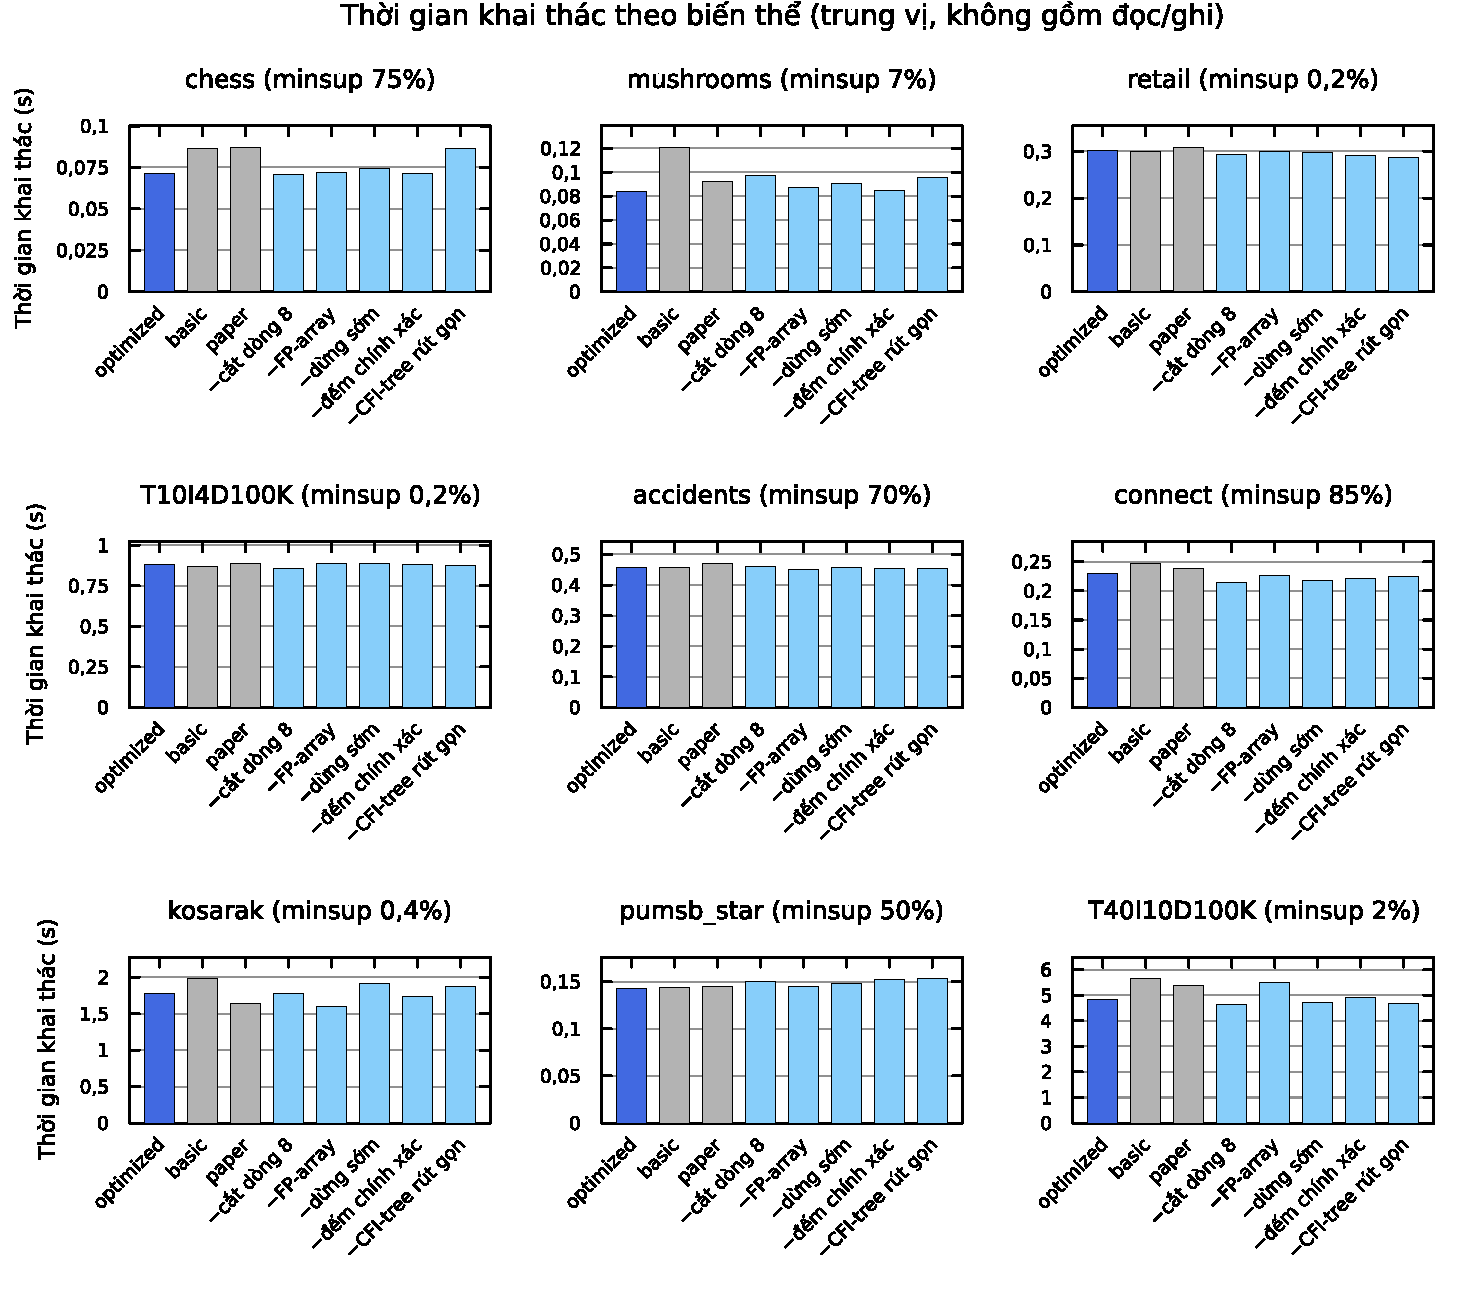
\includegraphics[width=0.82\textwidth]{time_variants_grid.pdf}
\caption{Thời gian khai thác của tám biến thể tại minsup giữa lưới (trung vị 3 lần đo, không gồm đọc và ghi file).}
\label{fig:time-variants}
\end{figure*}

\begin{table}[H]
\caption{Số tập đóng và thời gian (giây) theo độ dài giao dịch trung bình}
\label{tab:txlen}
\centering
\fittable{\columnwidth}{txlen_table}
\end{table}

% Đẩy hết bảng còn chờ của Phụ lục A (kể cả bảng rộng hai cột) ra trước khi sang Phụ lục B
\clearpage
\section{Dữ liệu và phương pháp đo}
\label{app:data}

\textbf{Chuẩn hóa dữ liệu.} Hai CSDL FIMI có mã item bắt đầu từ 0 (pumsb\_star và T40I10D100K) được ánh xạ mỗi item
$i$ thành $f(i)=i+1$. Phép ánh xạ một-một này bảo toàn nội dung giao dịch, support và tính đóng của các itemset
($\operatorname{supp}_D(X)=\operatorname{supp}_{f(D)}(f(X))$), nên sau chuẩn hóa cả chín CSDL chỉ chứa item có mã
nguyên dương. Quá trình chuẩn hóa chỉ thay đổi cách biểu diễn, không loại bỏ các giao dịch trùng nội dung, nhằm bảo
toàn support của các itemset.

\textbf{Phiên bản mushrooms.} Bản SPMF có 8\,416 giao dịch nhưng chỉ 8\,124 giao dịch phân biệt về nội dung, tương
ứng 292 lượt giao dịch lặp. Bản FIMI có đúng 8\,124 giao dịch, bằng số mẫu của UCI Mushroom~\cite{uci_mushroom}. Do
hai bản mã hóa item khác nhau, nhóm thống nhất dùng bản FIMI cho toàn bộ thực nghiệm.

\textbf{Độ biến thiên.} Mức biến thiên giữa 3 lần đo của mỗi cấu hình được tính bằng khoảng biến thiên tương đối
(\textit{relative range})
\begin{equation}
V=\frac{T_{\max}-T_{\min}}{T_{\min}}\times 100\%.
\label{eq:relrange}
\end{equation}
Trên 56 cấu hình minsup, trung vị của $V$ là 5{,}2\% với nhóm và 4{,}5\% với SPMF, tỉ lệ cấu hình có $V \le 20\%$ là
95\% (53/56) với nhóm và 93\% (52/56) với SPMF. Trên thực nghiệm ablation (72 tổ hợp CSDL và biến thể), trung vị của
$V$ đối với thời gian khai thác là 4{,}8\%. Chỉ ở một cấu hình (T40I10D100K 5\%), khoảng giá trị của 3 lần đo hai
phía chồng lên nhau.

\textbf{Phân tích độ nhạy.} Khi tính lại $r = T_{\text{nhóm}}/T_{\text{SPMF}}$ bằng giá trị nhỏ nhất thay cho
trung vị trên 78 cấu hình (56 cấu hình minsup, 10 cấu hình khả năng mở rộng, 12 cấu hình độ dài giao dịch), tính trên
số liệu chưa làm tròn, 76/78 cấu hình giữ nguyên nhóm. Hai cấu hình đổi nhóm là T10I4D100K 0{,}2\% ($r$ là 1{,}16 theo
giá trị nhỏ nhất và 1{,}08 theo trung vị) và kosarak 0{,}4\% (0{,}78 và 0{,}98). Một cấu hình đổi phía quanh 1 nhưng
vẫn nằm trong vùng gần tương đương (tập con 25\% của retail, minsup 0{,}05\%: 1{,}01 và 0{,}97). Mức thay đổi tương đối
lớn nhất của $r$ là 39\% (độ dài giao dịch 15, minsup 0{,}5\%: 0{,}22 và 0{,}31), cả hai giá trị đều thuộc nhóm nhanh
hơn.

\textbf{Dữ liệu tổng hợp theo độ dài giao dịch.} Một bộ 10\,000 giao dịch nền, mỗi giao dịch 32 item, được sinh với
seed 2026. Miền 500 item được chia thành 200 pattern 4 item (125 pattern rời nhau và 75 pattern chọn ngẫu nhiên),
pattern thứ $j$ có trọng số $1/(j+1)^{0{,}8}$. Mỗi giao dịch nền lấy 1, 2 hoặc 3 pattern (xác suất 25\%, 50\%, 25\%)
theo trọng số này rồi bổ sung item ngẫu nhiên đều cho đủ 32 item không trùng. CSDL có độ dài trung bình $\ell$ lấy
tiền tố của từng giao dịch nền với độ dài $\ell-2, \ldots, \ell+2$ (với $\ell=5$ là $\ell-1, \ldots, \ell+1$) chia đều
và xáo trộn, nên mỗi giao dịch ở mức dài chứa giao dịch tương ứng ở mức ngắn hơn.

\textbf{Máy thứ hai.} Thực nghiệm bộ nhớ (9 CSDL, 8 biến thể, 3 lần) được chạy trên máy Intel Core i5-13500H,
16\,GB RAM, cùng phiên bản Julia và Java, với phiên bản cài đặt trước khi có bộ đọc theo byte. Cả 216 lần chạy cho
cùng tập kết quả (cùng mã hash) như lần đo của Chương~\ref{sec:experiments}. Vì phiên bản cài đặt khác nhau, RAM và
thời gian trên máy này không được so với số liệu của Chương~\ref{sec:experiments}.

\section{Tái lập thực nghiệm}
\label{app:repro}

Mã nguồn ở \url{https://github.com/DRAGON-1312/FPClose}, dữ liệu ở
\url{https://huggingface.co/datasets/hytrang/fpclose-fim-benchmarks}. Phiên bản Julia, Java, SHA-256 của
\path{spmf.jar} và commit dùng khi đo được ghi tự động trong \path{results/ENVIRONMENT.md}. Các script:
\begin{itemize}
  \item \path{scripts/data_setup.jl}: tải chín CSDL, kiểm tra SHA-256, sinh tập con retail và dữ liệu tổng hợp.
  \item \path{scripts/verify_datasets.jl}: thống kê số giao dịch, số giao dịch phân biệt, số lượt lặp, miền mã item
        và offset của từng CSDL đã chuẩn hóa (kèm bản mushrooms của SPMF), ghi ra
        \path{results/dataset_validation.csv}.
  \item \path{scripts/reference_check.jl}: kiểm tra SPMF với FPclose gốc của kho FIMI.
  \item \path{scripts/run_benchmark_grid.jl}: chạy các thực nghiệm correctness, runtime, memory, scalability và
        txlen (lưới minsup ở \path{data/meta/benchmark_config.csv}), mỗi cấu hình 3 lần.
  \item \path{scripts/benchmark.jl}: đo bộ nhớ và thời gian khi bật, tắt từng tối ưu.
  \item \path{scripts/bench_reader.jl}: so bộ đọc theo dòng với bộ đọc theo byte, ghi ra
        \path{results/optimization/reader_bench.csv}.
  \item \path{scripts/sensitivity_analysis.jl}: so tỉ lệ thời gian nhóm/SPMF theo giá trị nhỏ nhất và trung vị
        trên 78 cấu hình, ghi ra \path{results/runtime/runtime_sensitivity.csv}.
  \item \path{scripts/fptree_size.jl}: đo tỉ lệ kích thước FP-tree (Bảng~\ref{tab:fptree}), ghi ra
        \path{results/fptree/fptree_size.csv}.
  \item \path{scripts/plot_results.jl}: vẽ mọi hình của Chương~\ref{sec:experiments} vào \path{results/figures/}
        (trung vị các lần đo, mô tả từng hình trong \path{results/figures/README.md}).
  \item \path{scripts/summarize_results.jl}: tổng hợp các bảng Markdown và CSV vào \path{results/summary/}.
  \item \path{scripts/make_figures.jl}: sinh các bảng LaTeX của báo cáo vào thư mục \path{tables/} (trung vị các
        lần đo).
\end{itemize}
Các script đo chạy từ thư mục gốc của repo theo dạng \texttt{julia --project=. scripts/<tên>.jl}, hai script vẽ và
tổng hợp dùng \texttt{--project=scripts/plot}, còn \path{make_figures.jl} dùng \texttt{--project=scripts/plots}. Riêng
\path{run_benchmark_grid.jl} mặc định chạy cả năm thực nghiệm và mất nhiều giờ, tham số \texttt{--only runtime} chỉ
chạy phần thời gian chạy. Các điểm khác bài báo gốc được tóm tắt ở Mục~\ref{sec:deviations} và ghi chi tiết trong
\path{docs/DEVIATIONS.md}.
    % Phụ lục: số liệu chi tiết của Chương 2, bắt đầu ở trang mới

\end{document}
